\chapter{Экспериментальные методы измерения коллективной анизотропии}

\section{Эксперимент HADES}

\subsection{Критерии отбора столкновений и рожденных частиц}

В работе приводятся результаты анализа экспериментальных данных, полученные из столкновений ядер Au+Au при энергии $E_{kin}=$1.23$A$~ГэВ а также ядер Ag+Ag при энергиях $E_{kin}=$1.23$A$ и 1.58$A$~ГэВ, полученные на установке HADES.
Всего было проанализировано около 100 миллионов столкновений Au+Au и по 500 миллионов столкновений для Ag+Ag при обеих энергиях.
Для исследования использовались столкновения разделенные по времени и восстановленной вершиной лежащей в области мишени.
Траектории заряженных частиц были отобраны на основании качества аппроксимации трека.
Для отбора первичных частиц использовался критерий на минимальное расстояние между ее траекторией и первичной вершиной. 

Для анализа использовались события столкновений тяжелых ядер, вершина которых лежала в следующих границах: $\sqrt{x_v^2+y_v^2}<3$~мм и $z_v \in (-60, 0)$~мм.
Распределение событий по восстановленной вершине показано на рис.~\ref{fig:hades_vertex}.
Слева представлено распределение восстановленной вершины по оси $z$, справа --- в плоскости $x-y$ для столкновений Au~+~Au при $E_{kin}=1.23A$~ГэВ.
\begin{figure}[ht]
    \begin{center}
        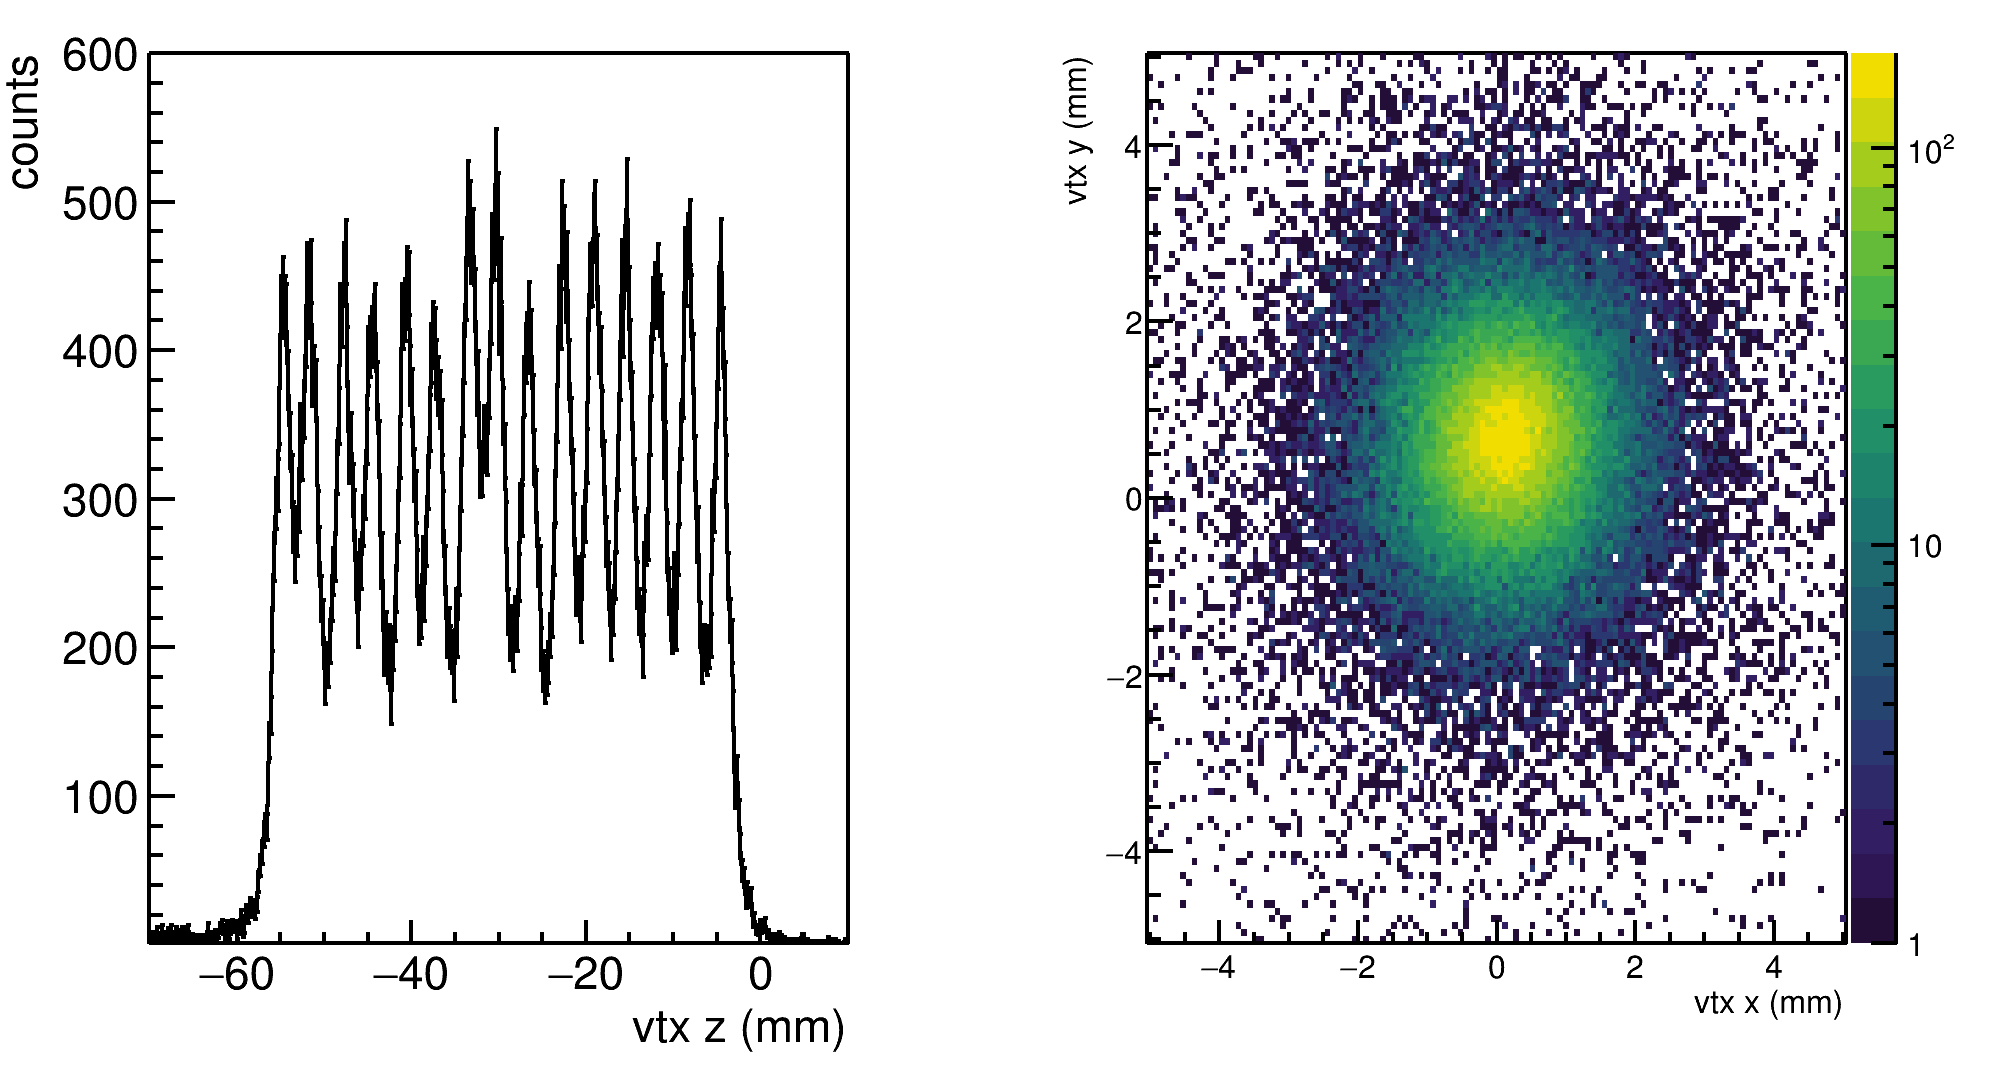
\includegraphics[width=0.95\linewidth]{images/hades_vertex.png}
        \caption{Слева: распределение восстановленной вершины по оси $z$, справа: в плоскости $x-y$ для столкновений Au~+~Au при $E_{kin}=1.23A$~ГэВ.}
        \label{fig:hades_vertex}
    \end{center}
\end{figure}

Для измерения направленного потока использовались траектории заряженных частиц которые были экстраполированы в вершину столкновения.
Траектории которые имели расстояние до восстановленной точки взаимодействия более 10~мм не использовались в анализе.
На рис.~\ref{fig:hades_dca} показано распределение восстановленных траекторий заряженных частиц по расстоянию наименьшего сближения с вершиной столкновения для Au~+~Au при $E_{kin}=1.23A$~ГэВ.
\begin{figure}[ht]
    \begin{center}
        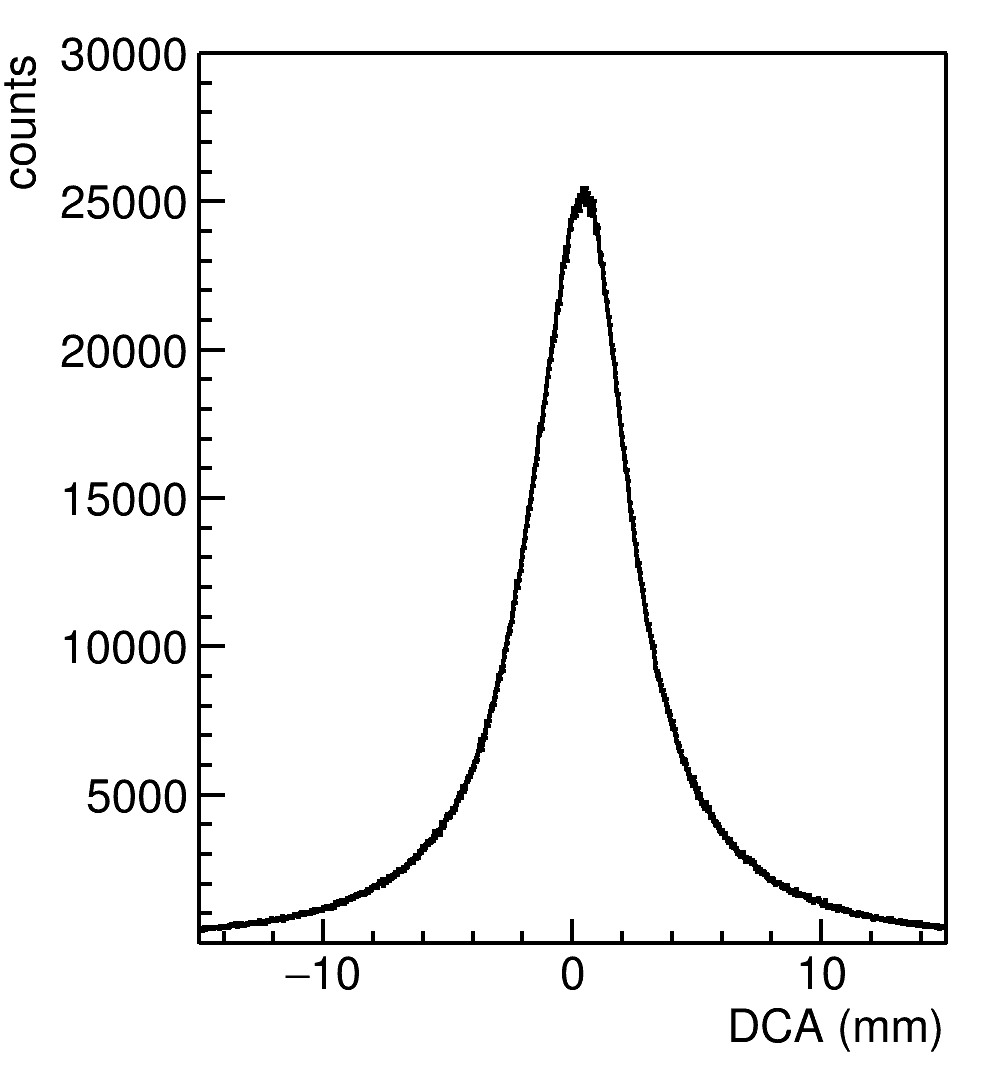
\includegraphics[width=0.55\linewidth]{images/hades_dca.png}
        \caption{Распределение восстановленных траекторий заряженных частиц по расстоянию наименьшего сближения с вершиной столкновения для Au~+~Au при $E_{kin}=1.23A$~ГэВ.}
        \label{fig:hades_dca}
    \end{center}
\end{figure}

\subsection{Определение центральности столкновения}

Центральность столкновений в эксперименте HADES была определена на основе числа срабатываний времяпролетной системы.
Регистрация столкновения выполняется по величине, пропорциональной множественности рожденных в столкновении частиц.
Триггер столкновения вырабатывается при превышении сигналом заданного порога.
Наиболее вероятными являются периферические столкновения, однако в силу малой множественности эти столкновения могут не вырабатывать необходимый сигнал для срабатывания триггера.
Это приводит к тому, что экспериментальное распределение множественности смещается в сторону более центральных столкновений.
Определеные классы центральности по такому распределению множественности тоже будут смещены.
К примеру, на рис.~\ref{fig:hades_multiplicity_comparison} представлено сравнение множественности срабатываний времяпролетной системы TOF+RPC для центрального триггера в столкновениях Au~+~Au при $E_{kin}=1.23$ и Ag~+~Ag при $E_{kin}=1.23$ и $E_{kin}=1.58A$~ГэВ.
Максимальная множественность в столкновениях ядер золота почти в 2 раза превышает максимальную множественность в столкновениях ядер серебра при одной энергии.
Для всех систем и энергий заметен спад в распределении для небольших значений множественности, который объясняется ограниченной эффективностью центрального триггера.
\begin{figure}[ht]
    \begin{center}
        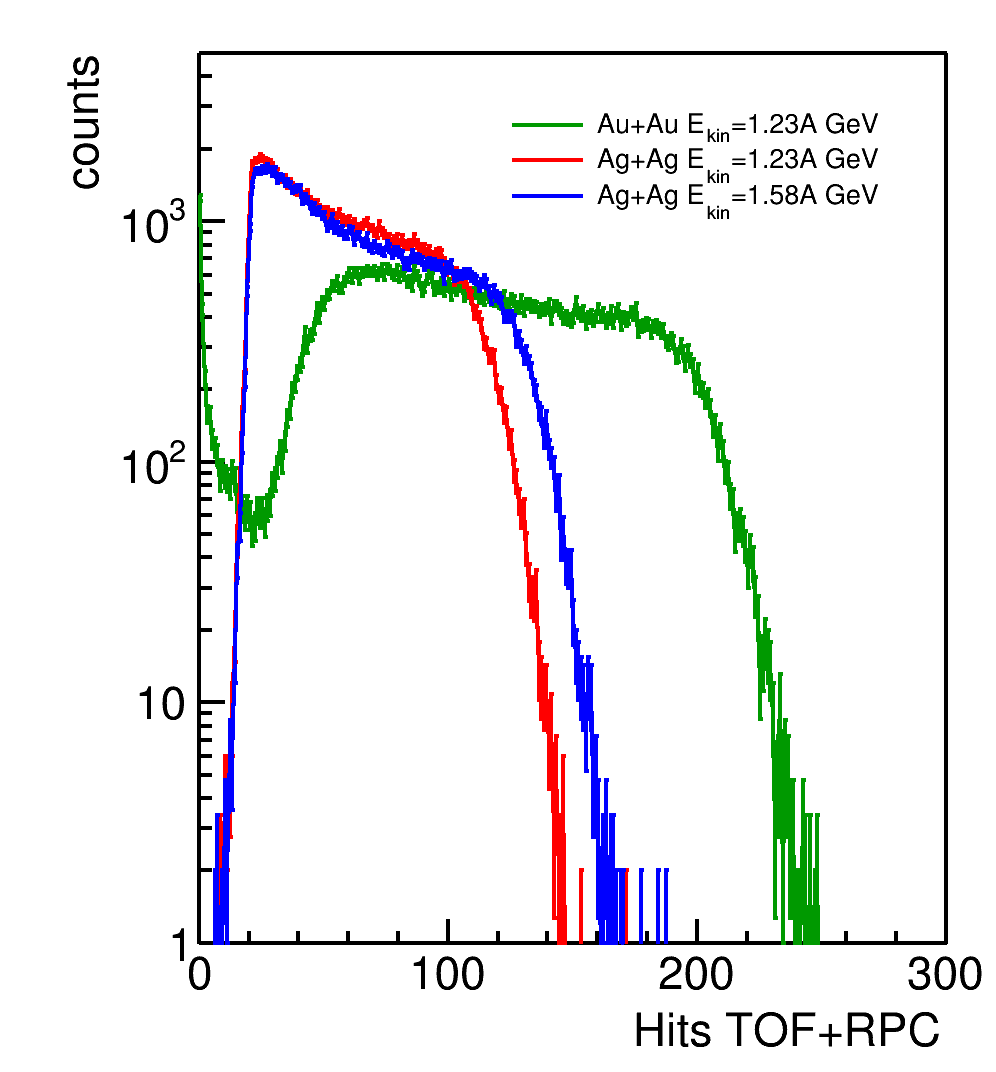
\includegraphics[width=0.55\linewidth]{images/hades_multiplicity_comparison.png}
        \caption{Сравнение множественности срабатываний времяпролетной системы TOF+RPC для центрального триггера в столкновениях Au~+~Au при $E_{kin}=1.23$ и Ag~+~Ag при $E_{kin}=1.23$ и $E_{kin}=1.58A$~ГэВ.}
        \label{fig:hades_multiplicity_comparison}
    \end{center}
\end{figure}
        
Для восстановления истинного распределения множественности с полным сечением неупругого взаимодействия и сопоставления классов центральности со средними значениями геометрических параметров в этих классах использовался метод МК-Глаубера~\cite{HADES:2017def}.
При помощи модели МК-Глаубера (параметры распределения Вудса-Саксона (\ref{eq:woods_saxon}): $R=6.55$~фм и $a=0.52$~фм~\cite{LandoltBornstein2004:sm_lbs_978-3-540-45555-4_81}) разыгрывалось число нуклонов-участников $N_{part}$ и число нуклон-нуклонных столкновений $N_{col}$.
Затем, варьируя параметры отрицального биномиального распределения $f$, $\mu$ и $k$, моделированное распределение множественности подгонялось под экспериментально измеренное распределение числа срабатываний времяпролётной системы TOF+RPC.
Восстановленное распределение множественности из связки МК-Глаубера и отрицательного биномиального распределения было разбито на классы центральности.
В каждом классе центральности из модели МК-Глаубера были извлечены средние значения геометрических параметров.

На рис.~\ref{fig:mc_glauber_auau} слева представлено распределение множественности срабатываений системы TOF-RPC в сеансе Au~+~Au при энергии 1.23$A$~ГэВ. Макрерами разных цветов обозначены данные, собранные с различными триггерами: "min-bais" --- триггер минимального смещения множественности и "central" --- триггер центральных событий.
Красная линия обозначает восстановленное методом МК-Глаубера распределение множественности с полным сечением.
Вертикальные линии обозначают границы классов центральности по множественности.
Для триггера центральных событий (зеленые маркеры) наблюдается хорошее согласие с восстановленной множественностью (красная линия) для классов центральности 0-30\%.
Триггер минимального смещения множественности (синие маркеры) эффективен для классов центральности 0-60\%.
Справа представлено распределение столкновений по множественности и прицельному параметру из модели МК-Глаубера. 
Горизонтальными пунктирными линиями обозначены границы классов центральности.
Для каждого из классов центральности было рассчитано среднее значение прицельного параметра.

\begin{figure}[ht]
\begin{center}
    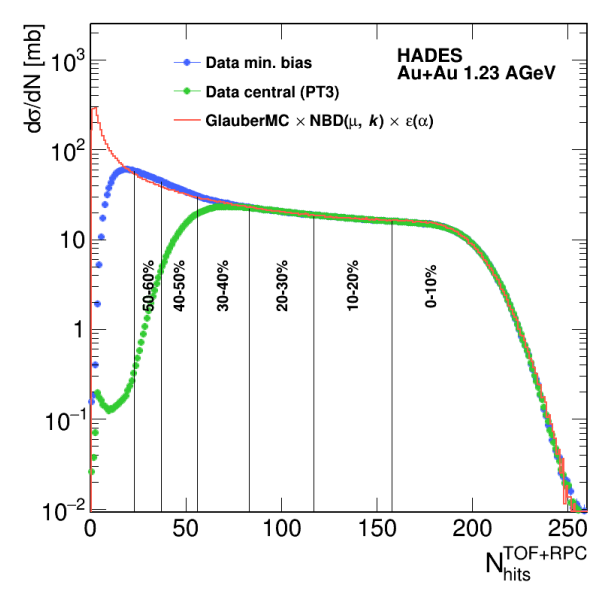
\includegraphics[width=0.45\linewidth]{images/mc_glauber_auau_mult.png}
    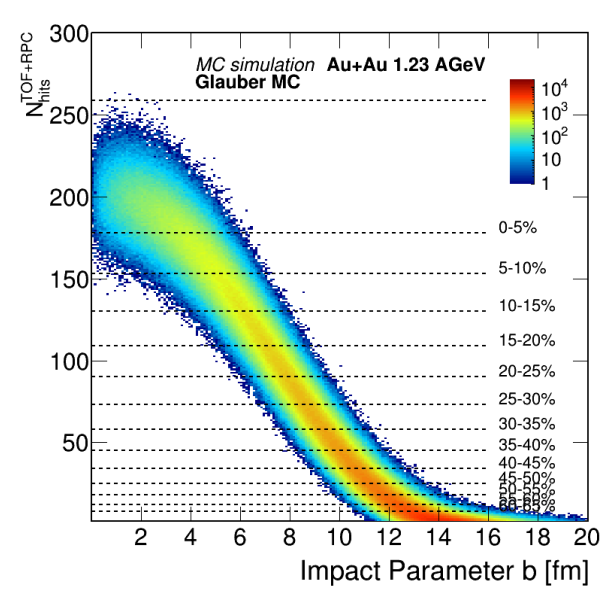
\includegraphics[width=0.45\linewidth]{images/mc_glauber_auau_b_mult.png}
    \caption{Слева: распределение множественности срабатываений системы TOF-RPC в сеансе Au~+~Au при энергии 1.23$A$~ГэВ. Справа: распределение разыгранной множественности методом МК-Глаубера и прицельного параметра для столкновений Au~+~Au при энергии 1.23$A$~ГэВ.}
    \label{fig:mc_glauber_auau}
\end{center}
\end{figure}

\subsection{Идентификация протонов времяпролётным методом}

Для измерения времени пролёта, установка HADES оборудована времяпролётными системами TOF и RPC, которые располагаются за трекинговой системой (см. рис.~\ref{fig:hades_bmn_layouts}).
Детектор TOF состоит из сцинтиляционных стержней, ориентированных радиально.
Детекторная подсистема RPC представляет из себя набор резистивных камер.
Идентификация частиц проводилась одновременно времяпролётным методом и по энерговыделению в камерах MDC.
На рис.~\ref{fig:hades_pid} представлено распределение заряженных частиц, зарегистрированных трекинговой системой HADES по относительной скорости $\beta$ и импульсу делённому на заряд $p/q$.
Используя соотношение:
\begin{equation}
    p = \frac{ m\beta }{ \sqrt{1-\beta^2} },
\end{equation}
где $p$ --- импульс частицы, $m$ --- ее масса, $\beta=v/c$, ее относительная скорость, можно рассчитать массу частицы.
%
\begin{figure}[ht]
    \begin{center}
    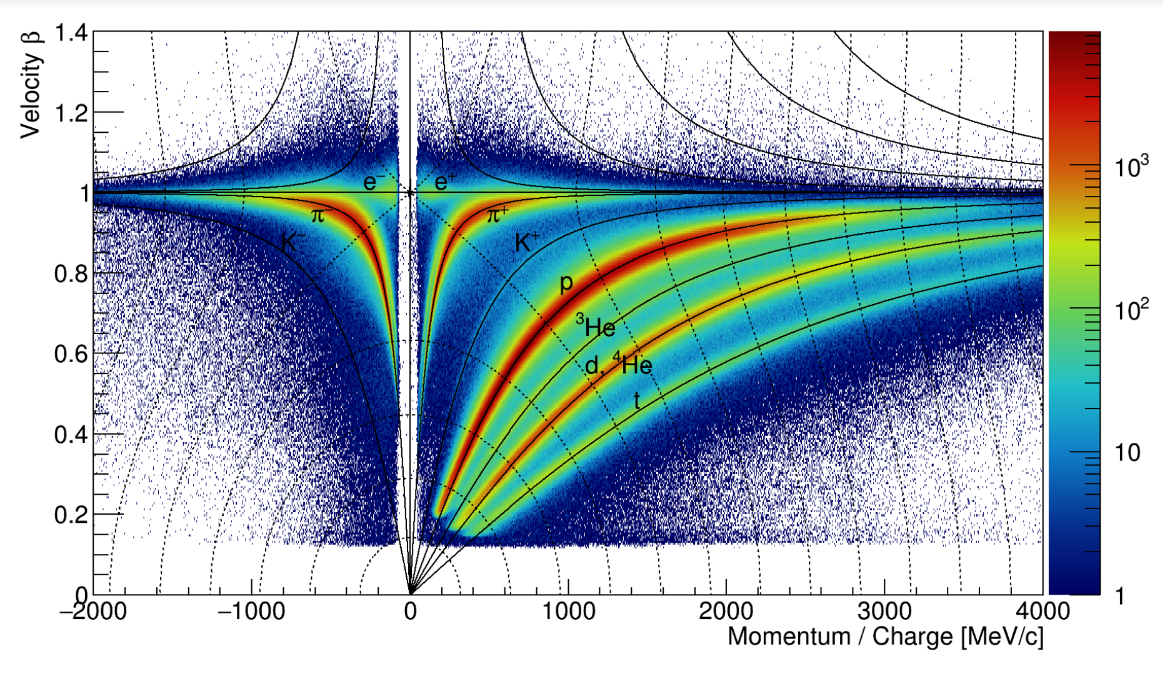
\includegraphics[width=0.95\linewidth]{images/hades_pid_plot.png}
    \caption{Распределение заряженных частиц, зарегистрированных трекинговой системой HADES по относительной скорости $\beta$ и импульсу делённому на заряд $p/q$.}
    \label{fig:hades_pid}
    \end{center}
    \end{figure}
    
Распределение заряженных частиц, зарегистрированных трекинговой системой HADES по квадрату массы $m^2$ и импульсу делённому на заряд $p/q$ представлено на рис.~\ref{fig:hades_m2_pq} (слева).
Ожидается, что массы рожденных частиц, измеренные времяпролётным методом будут распределены согласно нормальному распределению.
Среднее этого распределения для каждого типа частиц не должно зависить от импульса частицы, однако в эксперименте наблюдается сдвиг в сторону меньших значений для протонного пика.
Этот систмематический сдвиг может быть объяснён ошибкой при измерении частиц с малыми импульсами.
Большая кривизна траектории может приводить к ошибкам при ее реконструкции.
Ширина распределения для каждого вида частиц увеличивается с ростом импульса.
Этот эффект объясняется ограниченным разрешением времяпролётной системы, в которой при больших импульсах время пролёта восстанавливается с большей относительной ошибкой.
Каждый из пиков для разных типов частиц аппроксимируется функцией гаусса в узких диапазонах импульса.
Затем на основании этих аппроксимаций происходит отбор кандидатов в частицы для каждого типа.
Отобранные протоны представлены на рис.~\ref{fig:hades_m2_pq} (справа).
%
\begin{figure}[ht]
\begin{center}
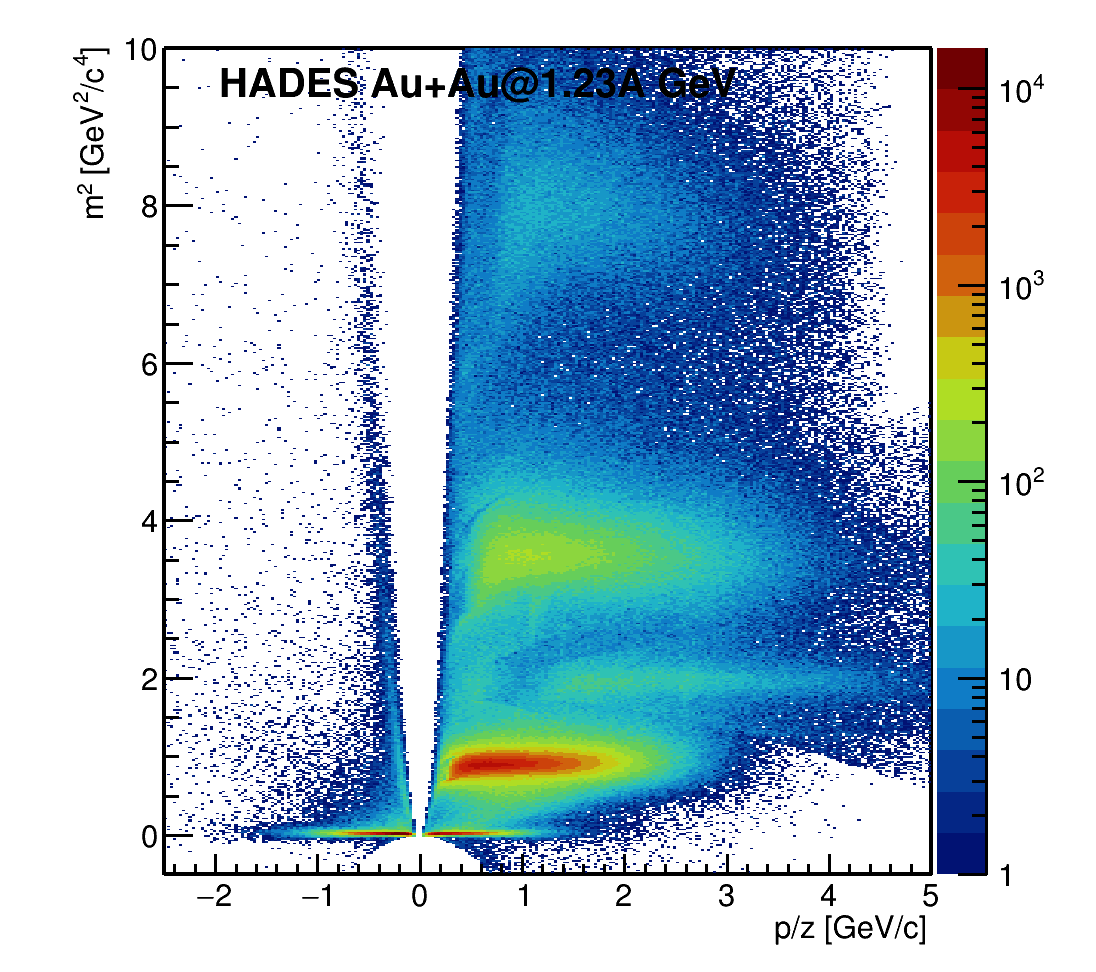
\includegraphics[width=0.45\linewidth]{images/au123_m2_vs_pq_all.png}
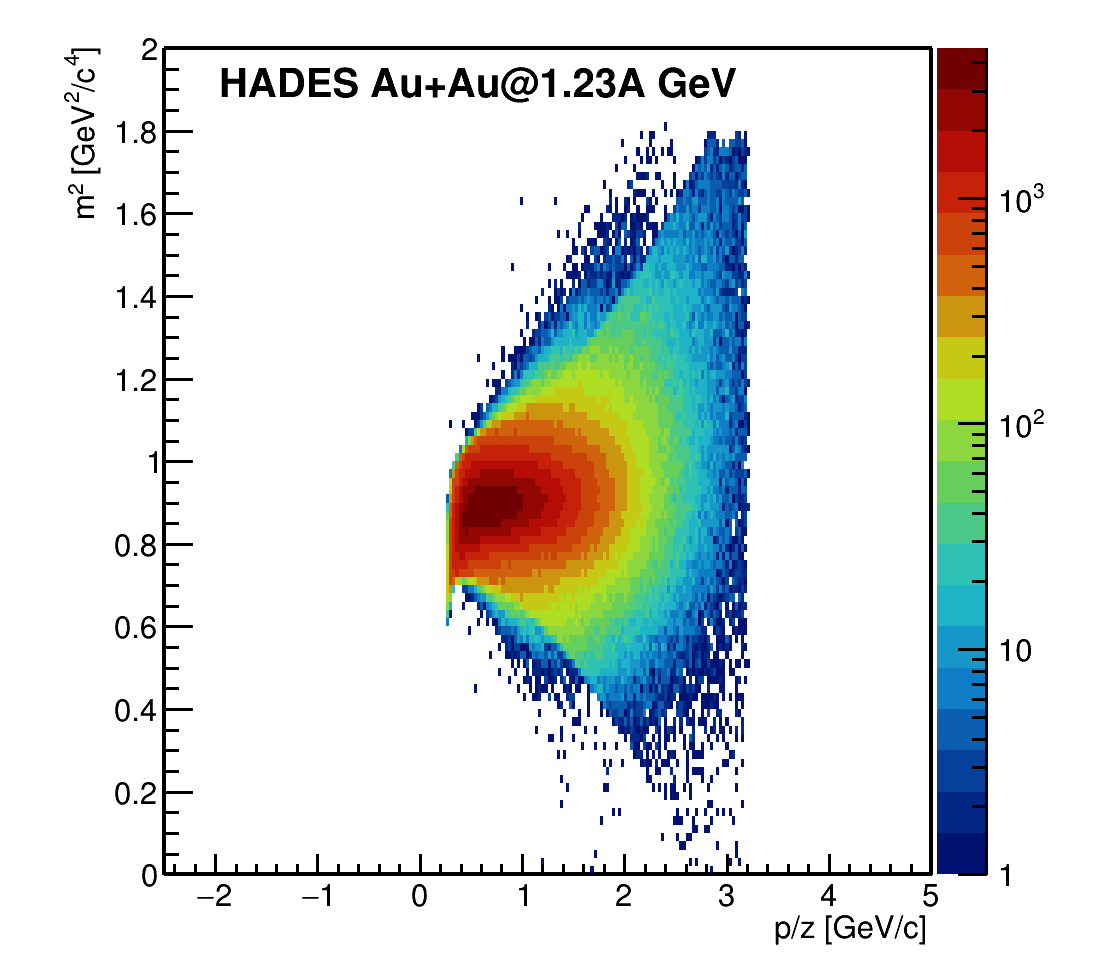
\includegraphics[width=0.45\linewidth]{images/au123_m2_vs_pq_protons.png}
\caption{Распределение заряженных частиц, зарегистрированных трекинговой системой HADES по квадрату массы деленному на квадрат заряда $m^2/q^2$ и импульсу делённому на заряд $p/q$: Для всех заряженных частиц (слева), для отобранных протонов (справа).}
\label{fig:hades_m2_pq}
\end{center}
\end{figure}

\subsection{Эффективность реконструкции протонов}

Эффективность реконструкции протонов была рассчитана при помощи Монте-Карло моделирования отклика детектора. 
В качестве входных данных использовалась физическая модель DCM-QGSM-SMM~\cite{Botvina:1994vj, Baznat:2019iom}.
Реалистичный отклик детекторов был смоделирован при помощи программного пакета GEANT3. 
Далее по модели отклика детектора была произведена реалистичная реконструкция.
Эффективность реконструкции определяется формулой:
\begin{equation}
    e(y, p_T) = \frac{ N_{rec}(y,p_T) }{ N_{sim}(y, p_T) },
\end{equation}
где $e(y, p_T)$ --- эффективность реконструкции для данных значений поперечного импульса ($p_T$) и быстроты ($y$), $N_{rec}$ --- число реконструированных частиц, $N_{sim}$ --- число смоделированных частиц.
На рис.~\ref{fig:hades_efficiency} представлена эффективность реконструкции протонов как функция быстроты ($y$) и поперечного импульса ($p_T$) для столкновений Au + Au при энергии $E_{kin}$=1.23$A$~ГэВ (слева), Ag + Ag при энергии $E_{kin}$=1.23$A$~ГэВ (посередине) и $E_{kin}$=1.58$A$~ГэВ (справа).
%
\begin{figure}[ht]
\begin{center}
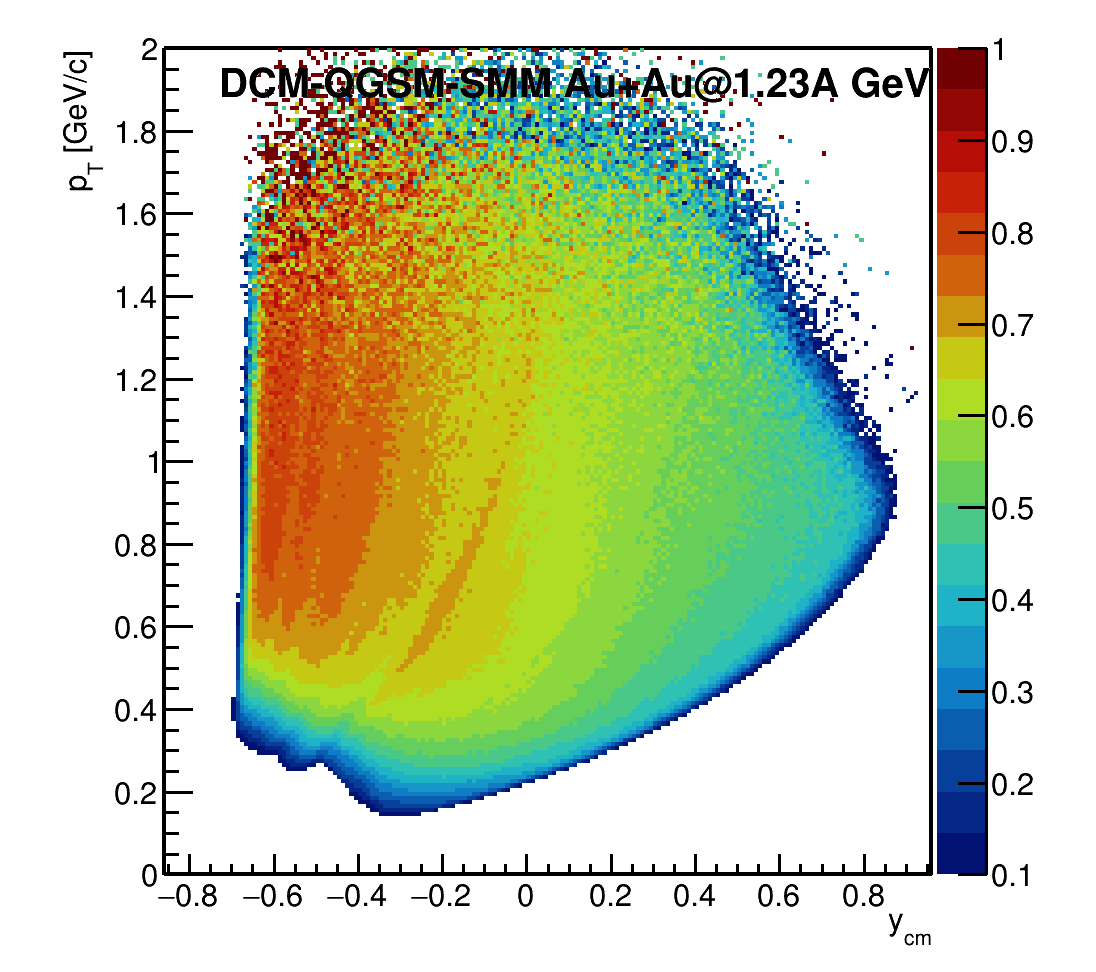
\includegraphics[width=0.3\linewidth]{images/au123_efficiency_y_pT.png}
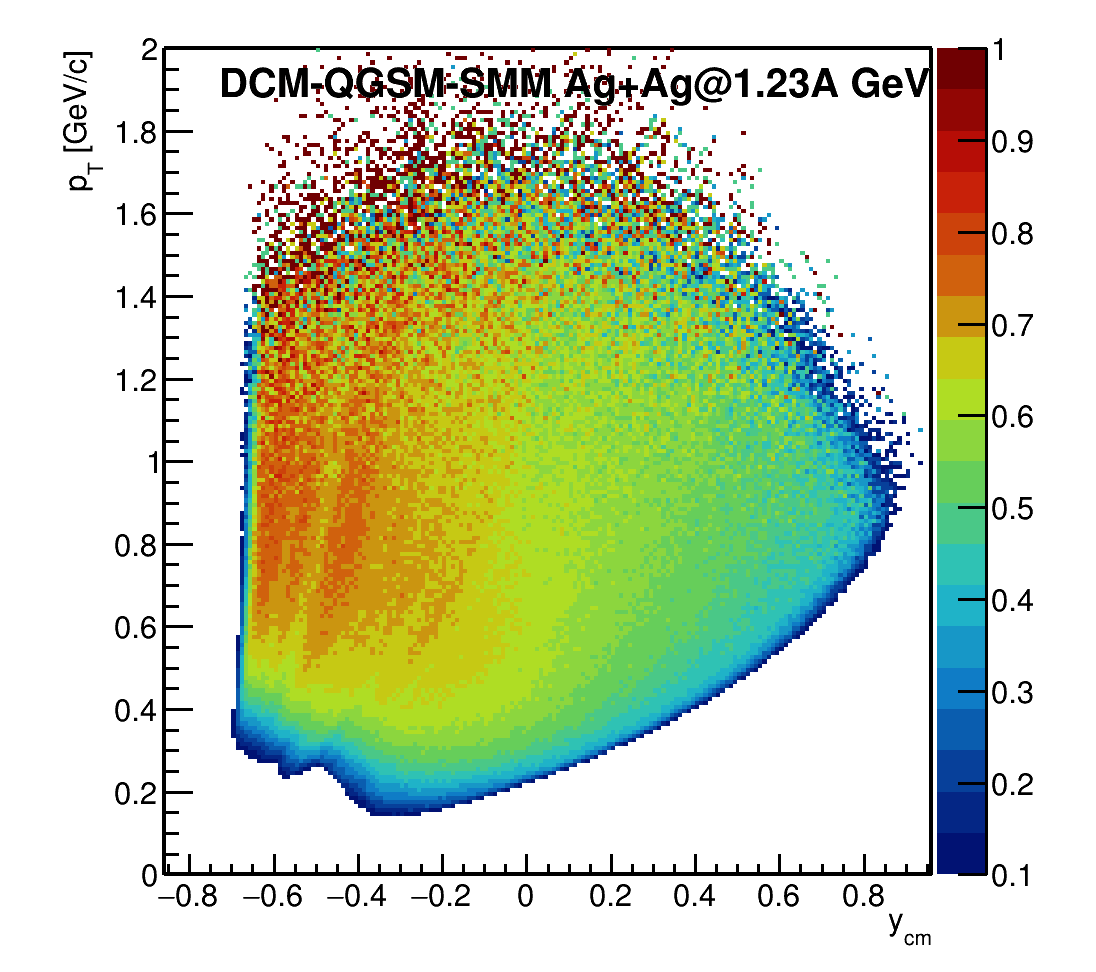
\includegraphics[width=0.3\linewidth]{images/ag123_efficiency_y_pT.png}
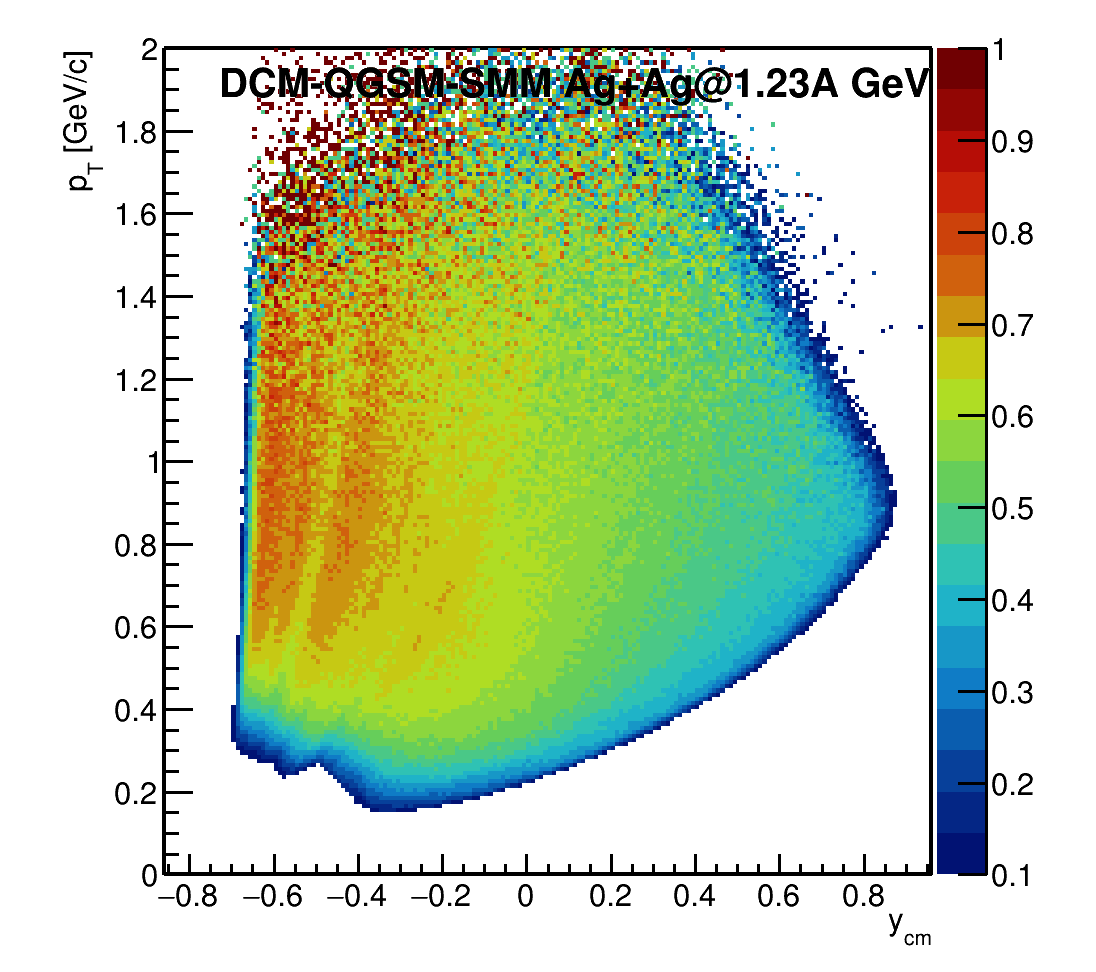
\includegraphics[width=0.3\linewidth]{images/ag158_efficiency_y_pT.png}
\caption{Эффективность реконструкции протонов как функция быстроты ($y$) и поперечного импульса ($p_T$) для столкновений Au + Au при энергии $E_{kin}$=1.23$A$~ГэВ (слева), Ag + Ag при энергии $E_{kin}$=1.23$A$~ГэВ (посередине) и $E_{kin}$=1.58$A$~ГэВ (справа). }
\label{fig:hades_efficiency}
\end{center}
\end{figure}

\subsection{Кинематические области используемые для определения $Q_1$ векторов}

Оценка плоскости симметрии в работе производилась по асимметрии распределения заряда спектаторов в детекторе FW. 
В качестве веса при вычислении $Q_1$-вектора использовался сигнал, зарегистрированный в модуле.
На рис.~\ref{fig:fw_signal} представлено распределение сигнала в модулях сцинтиляционной стенки FW для столкновений Au + Au при $E_{kin}$=1.23$A$~ГэВ (слева), Ag + Ag при $E_{kin}$=1.23$A$~ГэВ (посередине) и $E_{kin}$=1.58$A$~ГэВ (справа).
Наиболее выраженный пик отвечает заряду $Z=1$ (signal=100).
Также наблюдаются пики для зарядов $Z=2$ и $Z=3$.
События срабатывания модулей стенки с большими зарядами фрагментов редки.
%
\begin{figure}[ht]
\begin{center}
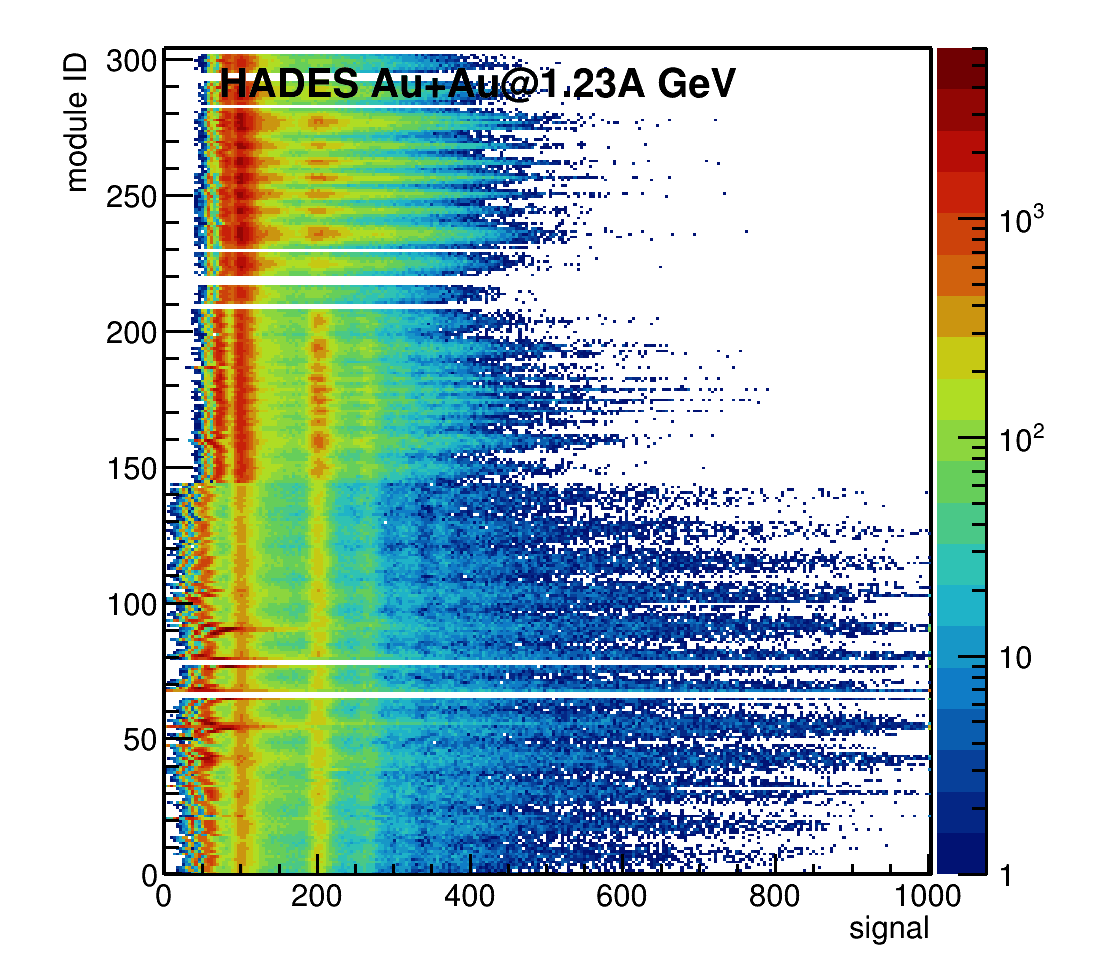
\includegraphics[width=0.3\linewidth]{images/au123_fw_modules.png}
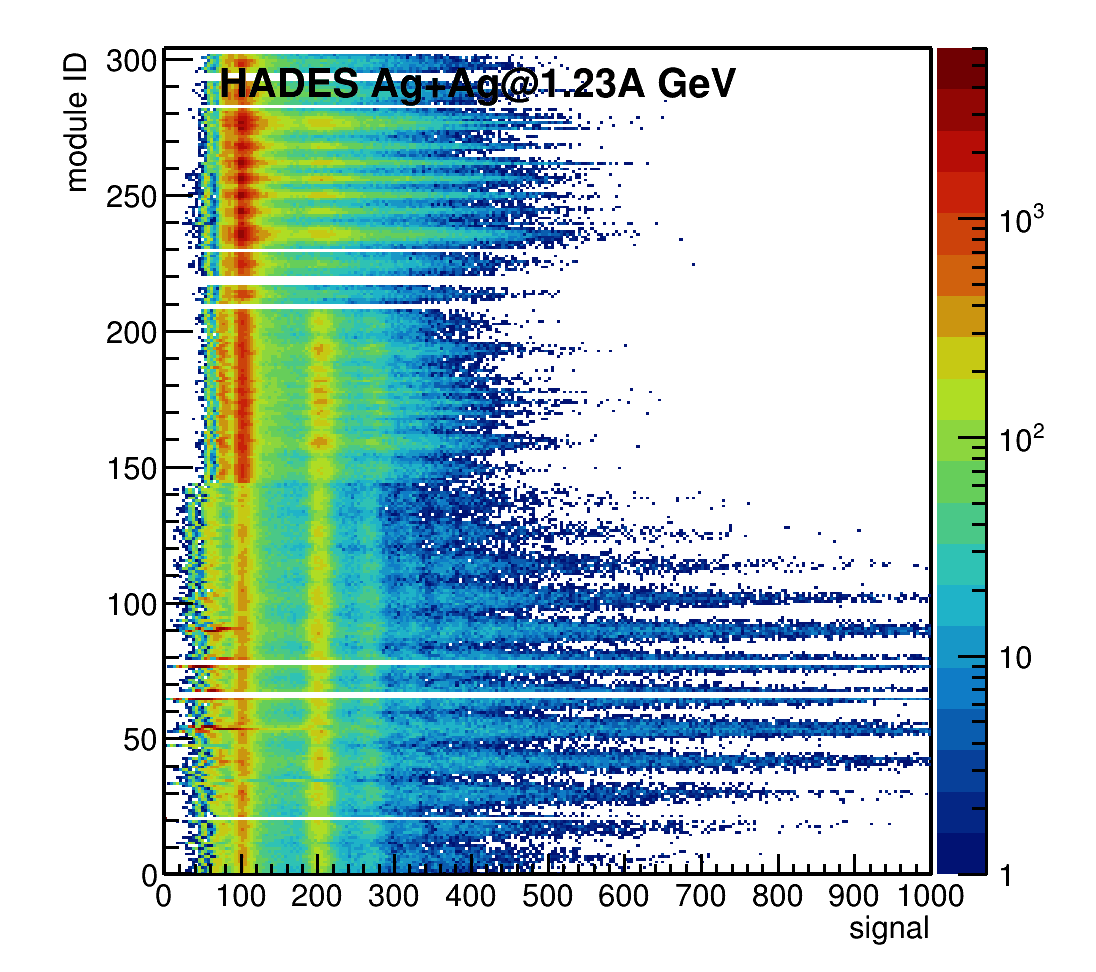
\includegraphics[width=0.3\linewidth]{images/ag123_fw_modules.png}
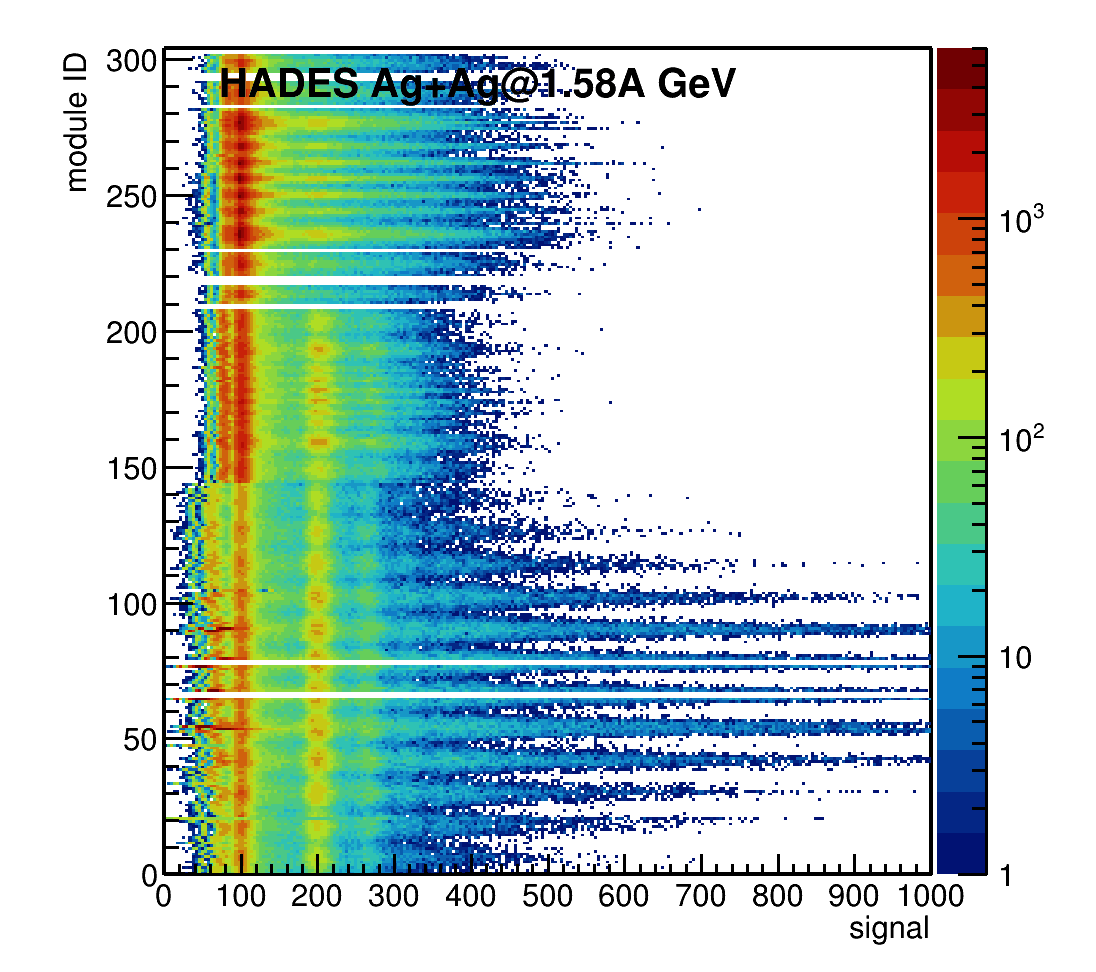
\includegraphics[width=0.3\linewidth]{images/ag158_fw_modules.png}
\caption{Распределение сигнала в модулях сцинтиляционной стенки FW для столкновений Au + Au при $E_{kin}$=1.23$A$~ГэВ (слева), Ag + Ag при $E_{kin}$=1.23$A$~ГэВ (посередине) и $E_{kin}$=1.58$A$~ГэВ (справа). }
\label{fig:fw_signal}
\end{center}
\end{figure}

$Q_1$-вектора из сцинтилляторной стенки вычислялись согласно формуле (\ref{eq:module_qn}) c $n=1$:
\begin{equation}
    \begin{align}
        Q_1^x = \frac{1}{C} \sum_{k=1}^N w_k \cos \phi_k \\
        Q_1^x = \frac{1}{C} \sum_{k=1}^N w_k \sin \phi_k,
    \end{align}
\end{equation}
где $\phi$ --- азимутальный угол и $w_k$ --- сигнал в $k$-м модуле. Номировочный коэффициент в случае метода скалярного произведения был равен $C=\sum_{k=1}{N} w_k$, а в случае метода плоскости события: $C = \sqrt{(Q_1^x)^2 + (Q_1^y)^2}$.
Модули детектора FW были разделены на 3 группы: центральные (W1), средние (W2) и периферические (W3).

Для оценки систематической ошибки вызванной непотоковыми корреляциями были введены 2 дополнительных $Q_1$-вектора из треков заряженных частиц.
Векторы $Q_1$ были построены из протонов c поперечным импульсом $p_T < 2.0$~ГэВ с быстротами $0.35 < y_{cm} < 0.55$ (Mf) и $-0.55 < y_{cm} < -0.35$ (Mb).
Для $Q_1$-векторов из треков заряженных частиц вычисления производились согласно формуле (\ref{eq:track_qn}):
\begin{equation}
    \begin{align}
        Q_1^x = \frac{1}{C} \sum_{k=1}^N \cos \phi_k \\
        Q_1^x = \frac{1}{C} \sum_{k=1}^N \sin \phi_k,
    \end{align}
\end{equation}
где $\phi_k$ --- азимутальный угол импульса $k$-й частицы. Для метода скалярного произведения нормировочный коэффициент $C=N$, в случае метода плоскости события: $C = \sqrt{(Q_1^x)^2 + (Q_1^y)^2}$.

Схематически расположение полученных векторов в плоскости $\eta$-$p_T$ изображено на рис~\ref{fig:hades_qvectors}.
%
\begin{figure}[ht]
\begin{center}
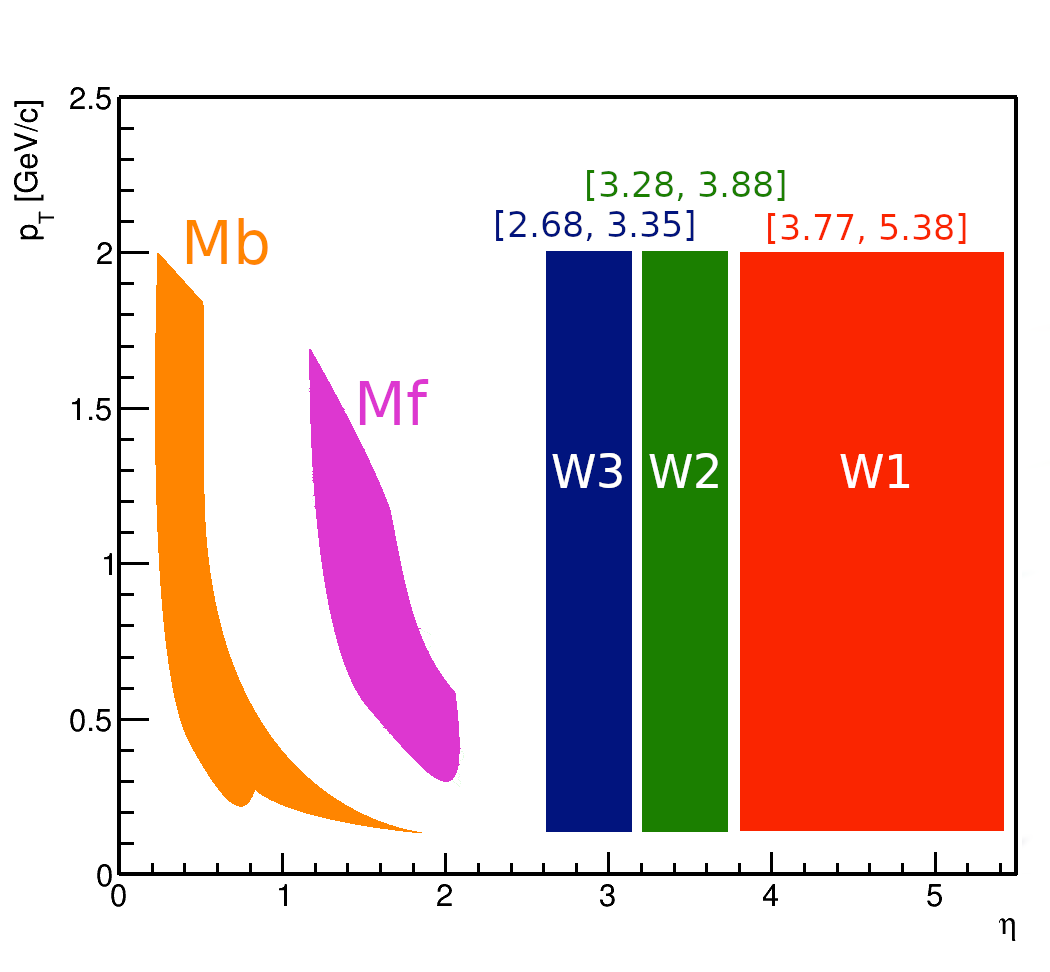
\includegraphics[width=0.75\linewidth]{images/eta_pt_qvectors.png}
\caption{Aксептанс по псевдобыстроте $\eta$ для подсобытий из FW и поперечному импульсу $p_T$ для подсобытий из MDC, использованных для расчета направленного потока протонов в столкновениях ядер золота и серебра.}
\label{fig:hades_qvectors}
\end{center}
\end{figure}
%


\section{Вычисление статистических погрешностей}

Некоторые $Q_n$-вектора участвуют одновременно в нескольких корреляциях, к примеру как в уравнении (\ref{eq:track_qn}).
Корреляции $\langle Q_1^a, Q_1^b \rangle$, $\langle Q_1^a, Q_1^c \rangle$ и $\langle Q_1^b, Q_1^c \rangle$ не являются независимыми измерениями, поэтому ошибки этих измерений скоррелированы.
В этом случае погрешность косвенных измерений, описываемая формулой ниже не является правильной:
\begin{equation}
    \delta f = \sqrt{ ( \frac{\partial f}{\partial a} \delta a )^2 + \frac{\partial f}{\partial b} \delta b )^2 + \frac{\partial f}{\partial c} \delta c )^2 },
\end{equation}
где $f$ --- некоторая величина, вычисленная при помощи измеряемых $a$, $b$ и $c$.

В данной работе для подавления корреляции ошибок использовался методо Bootstrap~\cite{Bohm:2010}.
Суть этого метода заключается в разбиении выборки на неэквивалентные поднаборы.
Тогда статистическая ошибка будет выражаться как среднеквадратичное отклонение распределения величины $f$, вычисленной в каждом поднаборе:
\begin{equation}
    \delta f = \sqrt{ \frac{ \sum_k w_k (f_k - \langle f \rangle )^ }{ \sum_k w_k - 1 } },
\end{equation}
где $w_k$ --- множественность данного поднабора, $f_k$ --- величина, вычисленная в данном поднаборе, $\langle f \rangle$ --- величина, вычисленная по всей выборке.


\subsection{Коррекция азимутальной анизотропии аксептанса детектора}

Азимутальный аксептанс трекинговой системы в зависимости от быстроты частицы приведён на рис.~\ref{fig:hades_phi_y}.
Азимутальный аксептанс трекинговой системы не является однородным, поскольку стыки секций трекинговой системы не способны регистрировать заряженные частицы.
Неоднородность увеличивается с ростом быстроты, поскольку площадь нечувствительного объёма по отношению к чувствительному уменьшаяется с ростом полярного угла $\theta$. 
%
\begin{figure}[ht]
\begin{center}
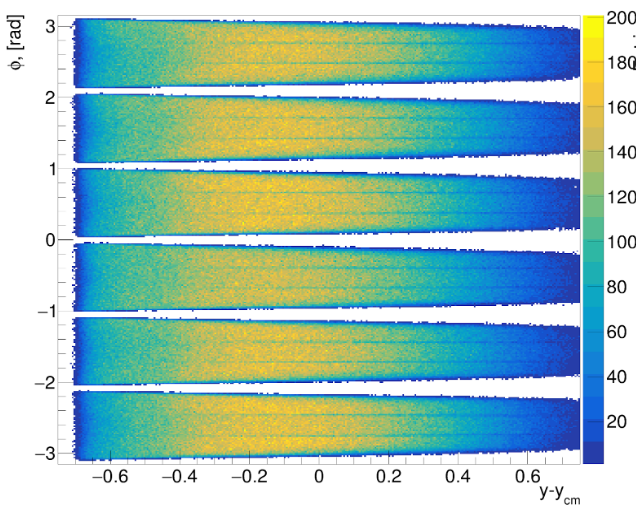
\includegraphics[width=0.55\linewidth]{images/hades_phi_y.png}
\caption{Азимутальный аксептанс трекинговой системы эксперимента HADES в зависимости от быстроты частицы.}
\label{fig:hades_phi_y}
\end{center}
\end{figure}

Для коррекции азимутальной неоднородноссти аксептанса был использован метод, предложенный в~\cite{Selyuzhenkov:2007zi}.
Данный метод основан на предположении, что азимутальное распределение частиц, рожденных в столкновении должно быть изотропным, поскольку угол плоскости реакции от события к событию распределен равномерно.
Азимутальная неоднородность чувствительного объема детектора вносит искажения в азимутальное распределение зарегистрированных частиц. 
Для коррекции на этот эффект, в статье~\cite{Selyuzhenkov:2007zi} вводятся поправки перецентровки, поворота и ремасштабирования. 
Схематически, действие этих поправок представлено на рис.~\ref{fig:qn_corrections}.
%
\begin{figure}[ht]
\begin{center}
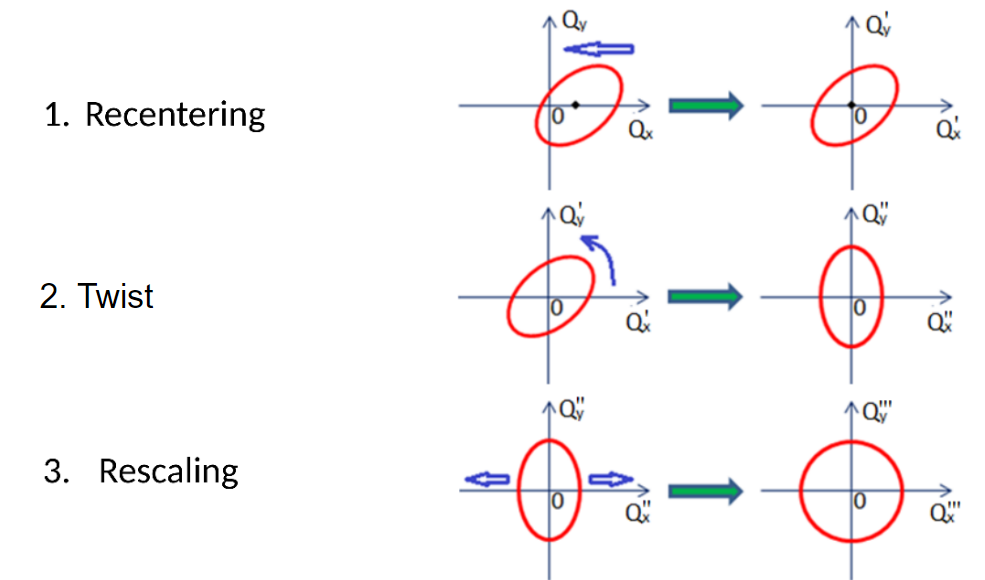
\includegraphics[width=0.75\linewidth]{images/qntools_corrections.png}
\caption{Схематическое изображение поправок предложенных в~\cite{Selyuzhenkov:2007zi}.}
\label{fig:qn_corrections}
\end{center}
\end{figure}
%

Описанные выше поправки применялись для коррекции азимутальной неоднородности аксептанса детектора мультидифференциально.
Для $Q_1$-векторов коррекции применялись в каждом классе центральности от 0\% до 40\% с шагом 5\%.
Для поправок на азимутальную неоднородность трекинга, коррекции на $u_1$-вектор применялись аналогично в каждом классе центральности а также дифференциально по поперечному импульсу $p_T$ и быстроте $y_{cm}$. 
Остаточные эффекты азимутальной неоднородности аксептанса в данной работе оцениваются как разность между корреляцией компонент $u_1$ и $Q_1$-векторов:
\begin{equation}
    \delta_{acc.} = | \langle x_1 X_1 \rangle - \langle y_1 Y_1 \rangle |,
\end{equation}
где $\delta_{acc.}$ --- остаточная ошибка после применения коррекций, $x_1$ и $y_1$, и $X_1$ и $Y_1$ --- компоненты $u_1$ и $Q_1$-векторов соответственно. 

Сравнение $v_1^{uncorr.}$, полученного с использованием различных компонент $u_1$ и $Q_1$-векторов, представлено на рис~\ref{fig:hades_uq_corr}. 
Направленный поток не корректирован на разрешение плоскости симметрии для оценки вклада неоднородного аксептанса трекинговой системы. 
После применения поправок на азимутальную анизотропию аксептанса, остаточный эффект составляет 2\%.
%
\begin{figure}[ht]
\begin{center}
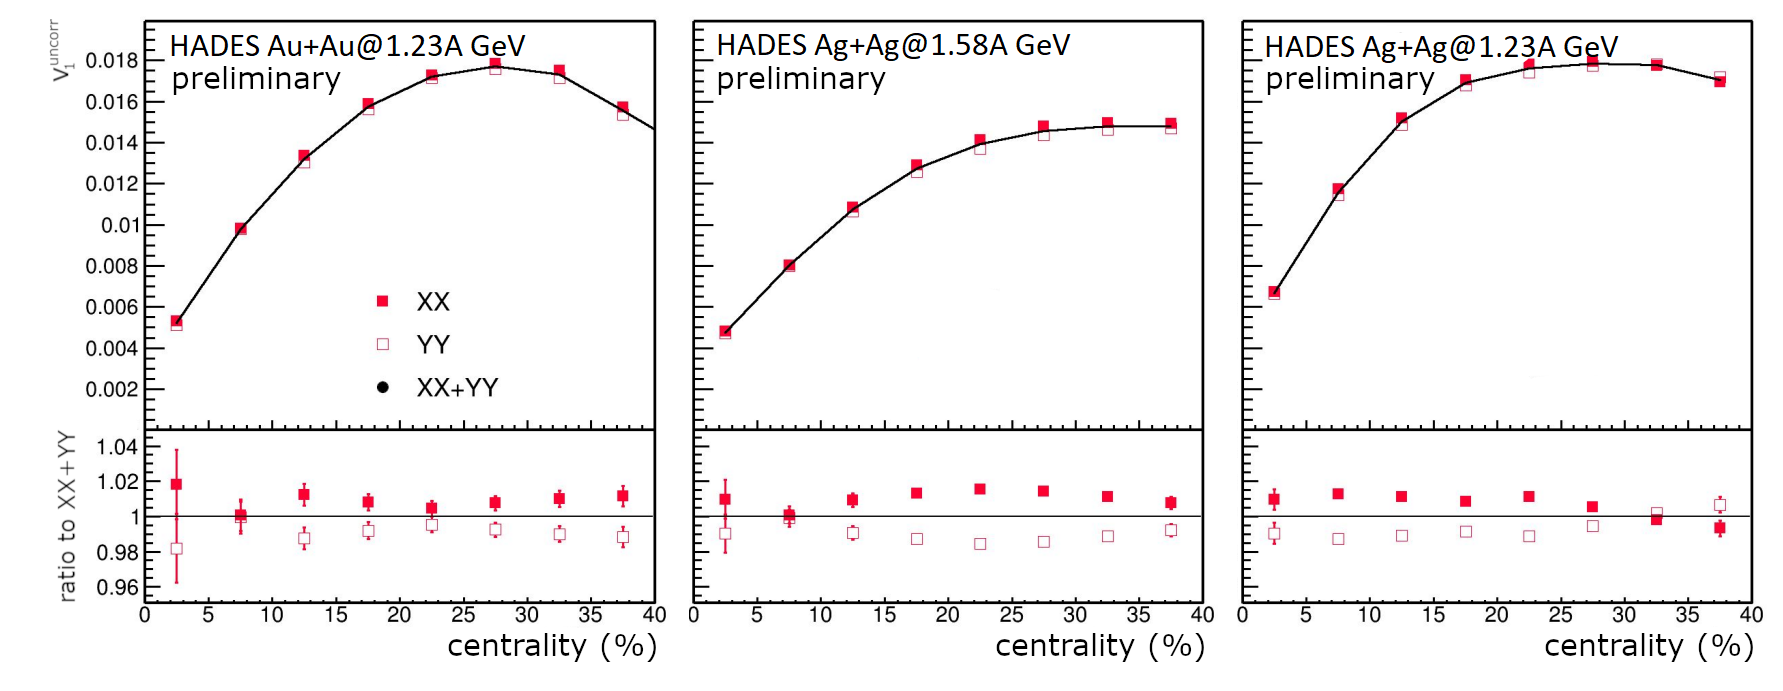
\includegraphics[width=0.75\linewidth]{images/hades_u1W1_centrality.png}
\caption{Сравнение компонент корреляции $\langle u_1 Q_1 \rangle$ после применения поправок на азимутальную неоднородность детектора для столкновений Au+Au@1.23A ГэВ (слева), Ag+Ag@1.23A ГэВ (посередине) и Ag+Ag@1.58A ГэВ (справа)}
\label{fig:hades_uq_corr}
\end{center}
\end{figure}
%

\subsection{Вычисление поравочного коэффициента разрешения $R_1$}

Для рассчета разрешения методом случайных подсобытий два вектора были определены из модулей детектора FW.
Модули были распределены в две группы случайным образом для каждого события.
Разрешение вычислялось согласно формуле (\ref{eq:r1_2sub}) с $n=1$:
\begin{equation}
    R_1 = \sqrt{ \langle Q_1^a, Q_1^b \rangle  }
\end{equation}

На рис.~\ref{fig:hades_R1_rs} представлено разрешение плоскости симметрии рассчитанное методом случайных подсобытий как функция центральности столкновения.
Основным недостатком данного метода является отсутствие возможности сравнить полученные значения с другими оценками разрешения плоскости симметрии.
%
\begin{figure}[ht]
\begin{center}
    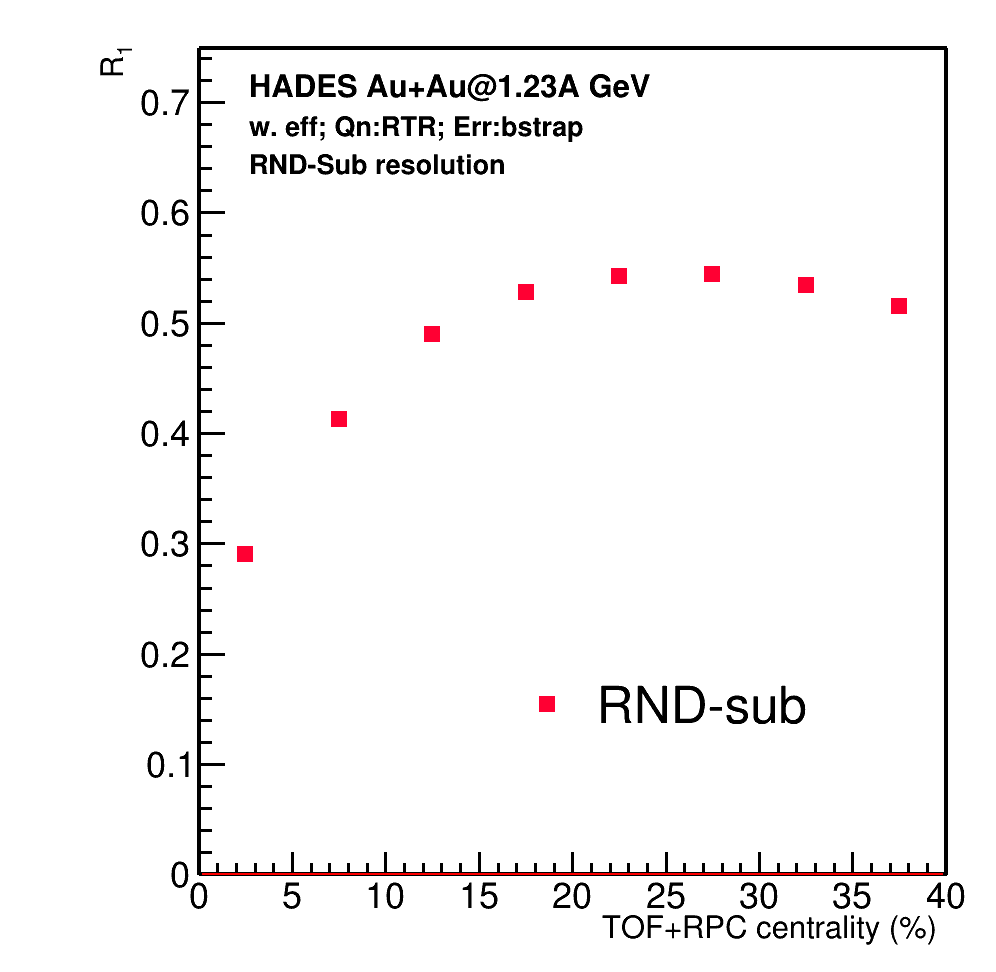
\includegraphics[width=0.3\linewidth]{images/R1_au123_rnd_centrality.png}
    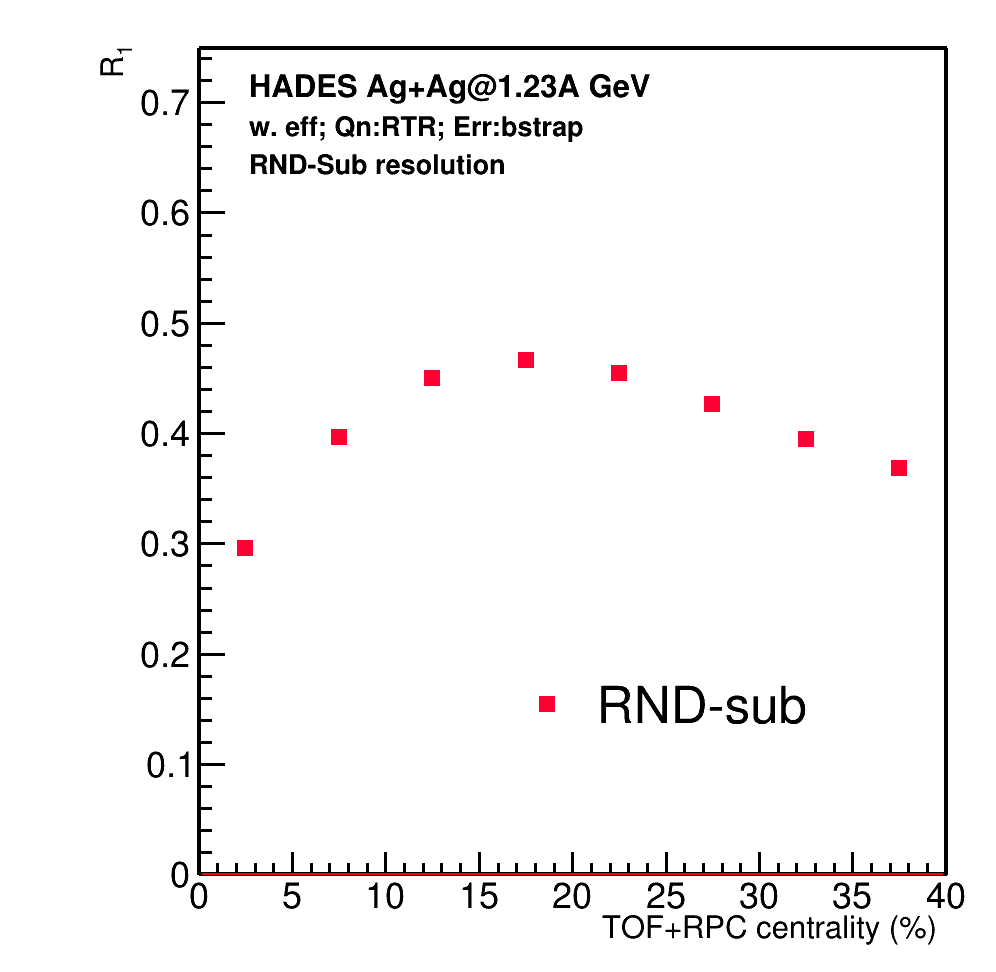
\includegraphics[width=0.3\linewidth]{images/R1_ag123_rnd_centrality.png}
    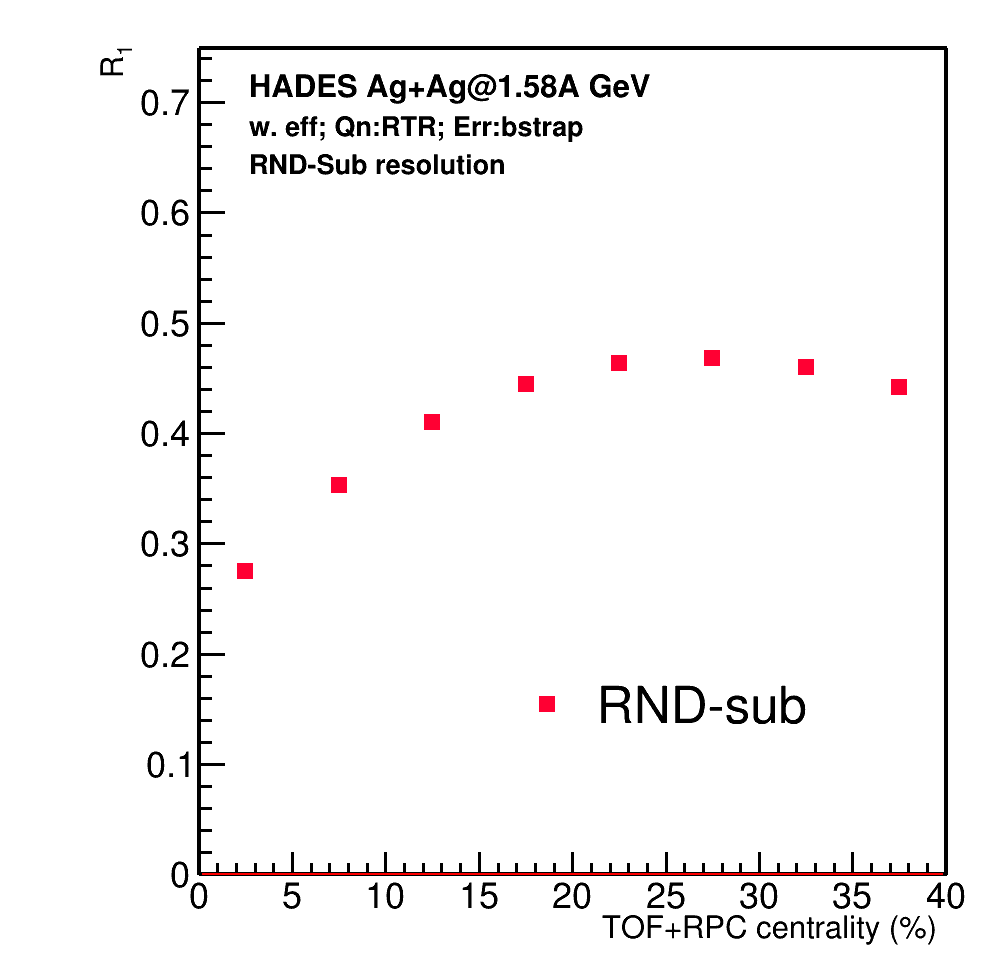
\includegraphics[width=0.3\linewidth]{images/R1_ag158_rnd_centrality.png}
    \caption{Разрешение плоскости симметрии рассчитанное методом случайных подсобытий как функция центральности столкновения.
    Слева: для столкновений Au + Au при $E_{kin}$=1.23$A$~ГэВ;
    посередине: для столкновений Ag + Ag при $E_{kin}$=1.23$A$~ГэВ; 
    справа: для столкновений Ag + Ag при $E_{kin}$=1.58$A$~ГэВ; 
    }
    \label{fig:hades_R1_rs}
\end{center}
\end{figure}
%

Вычисление разрешения методом трех подсобытий производилось согласно формуле (\ref{eq:r1_3sub}):
\begin{equation}
    R_1\{a(b,c)\}  =  \sqrt { \frac{ \langle Q_1^a Q_1^b \rangle \langle Q_1^a Q_1^c \rangle }{ \langle Q_1^b Q_1^c \rangle} }.
\end{equation}
Для расчета разрешения методом трёх подсобытий в работе введены 5 $Q_1$-векторов. 
Используя в методе трех подсобытий различные комбинации векторов, можно оценить остаточные эффекты из-за непотоковых корреляций. 
Очевидно, что разрешение плоскости симметрии, посчитанное с использованием различных комбинаций, должны совпадать, а возможная разница будет связана с эффектами не относящимися к коллективному движению частиц.
Исключая из анализа разрешение полученное при помощи комбинаций, в которых два или более векторов коррелируют по непотоковому каналу, можно значительно уменьшить вклад непотоковых корреляций в полученные результаты.
Таким образом, систематическая ошибка из-за эффектов, не связанных с коллективным движением частиц может быть рассчитана следующим образом:
\begin{equation}
    \delta_{NF} = R_1\{a(b,c)\} - R_1\{a(d,e)\},
\end{equation}
где $\delta_{NF}$ --- ошибка из-за непотоковых корреляций, а буквами от $a$ до $e$ обозначены различные $Q_1$-вектора.

Разрешение плоскости симметрии $W1$, полученное с использованием различных комбинаций $Q_1$-векторов, показано на рис~\ref{fig:hades_w1_combinations}.
Разрешение $R_1\{W1(W2,W3)\}$ заметно отличается от значений, полученных при помощи других комбинаций. 
Этот эффект может быть объяснён наличием непотоковых корреляций между парами $Q_1$-векторов $W1$ и $W2$, $W2$ и $W3$.
Эти векторы не имеют достаточного разделения по быстроте, поэтому в значительной степени могут быть подвержены непотоковым корреляциям. 
В столкновениях Ag+Ag при обеих энергиях, $R_1\{W1(Mf,Mb)\}$ также значительно отклоняется от среднего результата. 
Это может быть вызвано наличием корреляций из-за закона сохранения импульса между векторами $Mf$ и $Mb$. 
В столкновениях Au+Au этот эффект менее выражен в силу большей множественности рождённых частиц.
%
\begin{figure}[ht]
\begin{center}
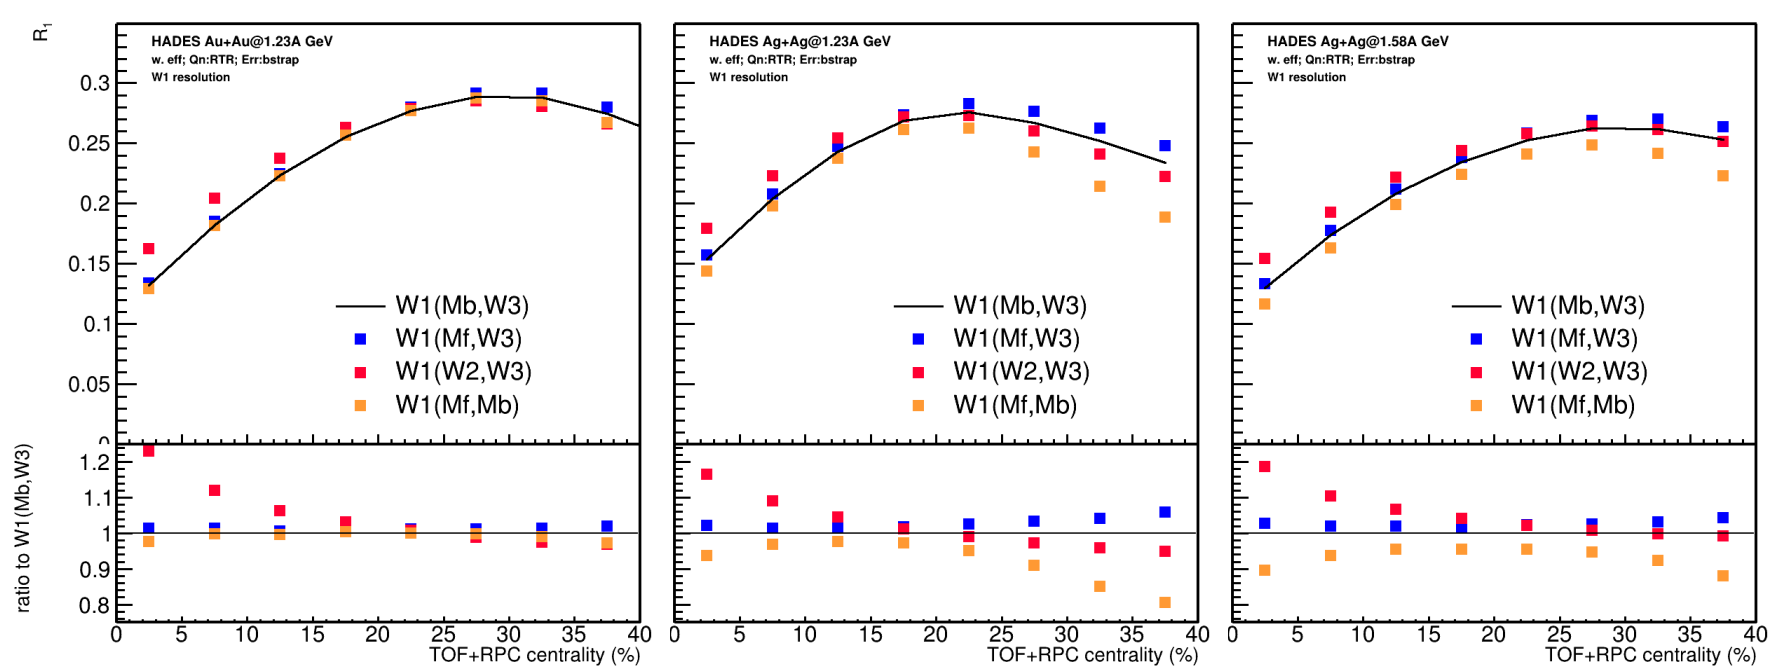
\includegraphics[width=0.75\linewidth]{images/W1_combinations.png}
\caption{Сравнение разрешений плоскости симметрии $W1$ полученное с использованием различных комбинаций $Q_1$-векторов для Au+Au@1.23A ГэВ (слева), Ag+Ag@1.23A ГэВ (посередине) и Ag+Ag@1.58A ГэВ (справа)}
\label{fig:hades_w1_combinations}
\end{center}
\end{figure}

\section{Оценка вклада непотоковых корреляций в значения $v_1$}

Направленный поток $v_1$ измерялся как проекция вектора частиц $u_1$ на плоскость симметрии $Q_1$, усредненная по частицам и событиям в данной области поперечного импульса $p_T$ и быстроты $y$:
\begin{equation}
    v_1(p_T, y) = \frac{ \langle u_1(p_T, y) Q_1 \rangle }{ R_1 },
\end{equation}
где $R_1$ --- разрешение плоскости симметрии для данного $Q_1$-вектора, а угловые скобки обозначают усреднение по всем частицам в данной кинематической области и всем событиям.

Для оценки систематики из-за непотоковых корреляций в полученных результатах $v_1$, был использован аналогичный метод, что и для разрешения плоскости симметрии. 
Для каждой плоскости симметрии, направленный поток может быть скорректирован на поправочный коэффициент разрешения рассчитанный с использованием различных комбинаций $Q_1$-векторов.
Сравнивая значения поправочного коэффициента, полученного при помощи различных комбинаций, можно оценить вклад непотоковых корреляций между $Q_1$-векторами.
Для проверки величины непотоковых корреляций между векторами частиц $u_1$ и вектором плоскости симметрии $Q_1$, можно сравнить значения $v_1$, полученные относительно различных плоскостей симметрии.
Таким образом, сравнивая направленный поток $v_1$, полученный относительно различных плоскостей симметрии и деленный на поправочный коэффициент разрешения, вычисленный с использованием различных комбинаций $Q_1$-векторов можно оценить вклад непотоковых корреляций в измеренные значения $v_1$.

На рис.~\ref{fig:hades_w1w3} представлен направленный поток протонов $v_1$, рожденных в столкновении Au+Au при энергии $E_{kin}=$1.23$A$~ГэВ, как функция центральности столкновения, измеренный относительно различных $Q_1$-векторов. 
Коррекция на поправочный коэффициент разрешения выполнена с использованием различных комбинаций $Q_1$-векторов.
Слева представлены значения $v_1$ протонов измеренные относительно внутреннего подсобытия W1, справа --- внешнего подсобытия W3 и подсобытия из треков заряженных частиц Mf. 
Результаты для комбинаций подсобытий, разделенных по быстроте, таких как например, $W1(Mf,W3)$ и $W1(Mb,W3)$ согласуются между собой в пределах 2\%, за исключением наиболее центральных событий. 
Результаты для $v_1$, полученные с использованием комбинации не разделенных по быстроте $Q_1$-векторов (например $W1(W2,W3)$) значительно отличаются.
Направленный поток протонов $v_1$, измеренный относительно различных плоскостей симметрии $W1$ и $W3$, так же согласуется в пределах 2\%.
Значения $v_1$ протонов, полученные относительно треков заряженных частиц $Mf$, систематически отличается от результатов полученных относительно плоскостей $W1$ и $W3$. 
Отсюда можно сделать вывод о недостаточном разделении по быстроте между подсобытием $Mf$ и рожденными протонами, для которых производились измерения.
В то же самое время, разделение по быстроте между зарегистрированными протонами и подсобытиям $W1$ и $W3$ достаточно.
В дальнейшем, в качестве значений $v_1$ протонов будет использовано среднее по всем комбинациям $Q_1$-векторов, разделенных по быстроте.
%
\begin{figure}[ht]
\begin{center}
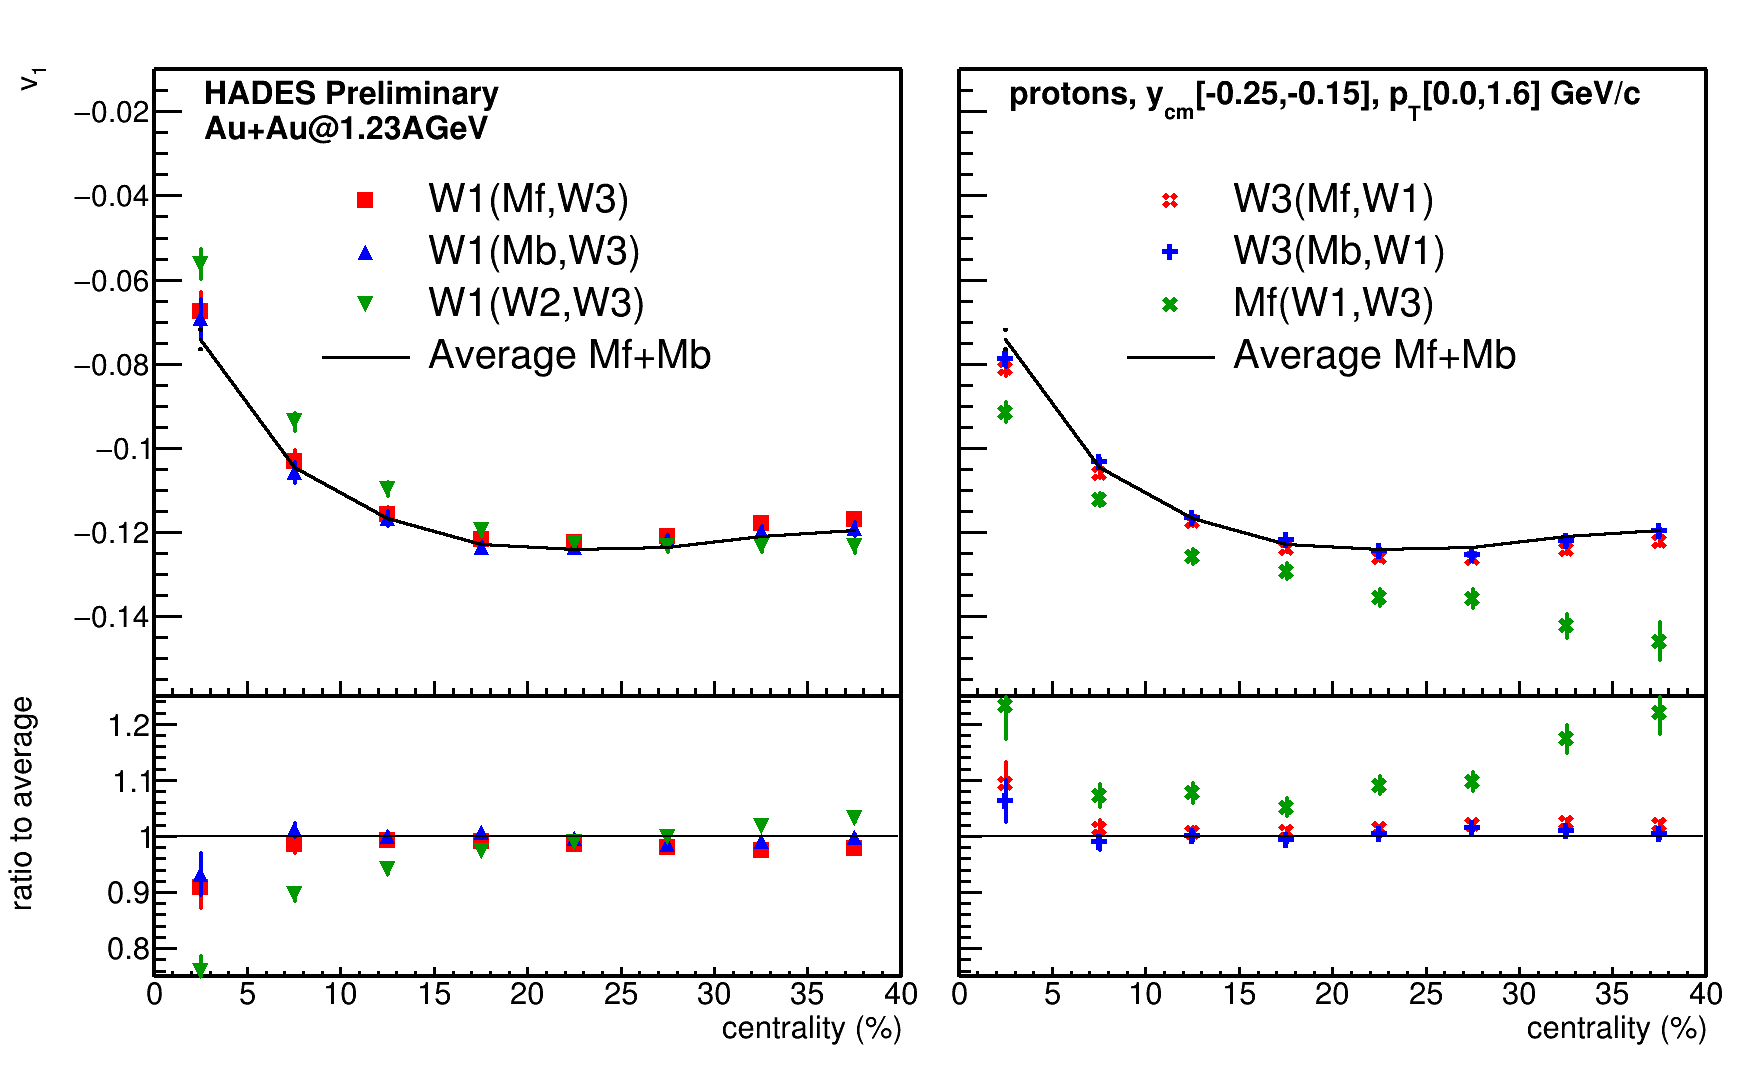
\includegraphics[width=0.75\linewidth]{images/W1AndW3Nucleus.png}
\caption{Направленный поток протонов $v_1$ рожденных в столкновении Au+Au при энергии $E_{kin}=$1.23$A$~ГэВ как функция центральности столкновения, измеренный при помощи различных комбинаций $Q_1$-векторов. Слева представлены значения $v_1$ протонов измеренные относительно внутреннего подсобытия W1, справа --- внешнего подсобытия W3 и подсобытия из треков заряженных частиц Mf. Черной линией представлено среднее результатов полученных при помощи разделенных по быстроте комбинаций.}
\label{fig:hades_w1w3}
\end{center}
\end{figure}

\subsection{Сравнение методов плоскости события и скалярного произведения}

Измерения направленного потока в~\cite{HADES:2020lob} были выполнены используя метод плоскости события, в котором вводится нормировка модуля $Q_1$-вектора на единицу. 
Такая нормировка может приводить к тому, что измеренные значения $v_1$, в зависимости от числа частиц, которые были использованы для построения $Q_1$-вектора, будут лежать между двумя пределами: $(\langle v_1 \rangle , \sqrt{ \langle v_1^2 \rangle })$.
В то же самое время, метод плоскости события в независимости от числа частиц даёт имзеренный $v_1 = \sqrt{ \langle v_1^2 \rangle }$.
Для оценки возможной систематики, связанной с этим методом измерения $v_1$, направленный поток был рассчитан методом скалярного произведеления.
Сравнение результатов полученных этими двумя методами позволит оценить вклад нелинейной зависимости $v_1\{EP\}$ от аксептанса установки и реального значения $v_1$.

На рисунке~\ref{fig:hades_ep_vs_sp} представлен направленный поток протонов рожденных в столкновениях Au+Au при энергии $E_{kin}=$1.23$A$~ГэВ как функция центральности, измеренный методом плоскости события и скалярного произведения. 
Значения $v_1$, полученные различными методами, хорошо согласуются между собой с учетом статистической ошибки. 
%
\begin{figure}[ht]
\begin{center}
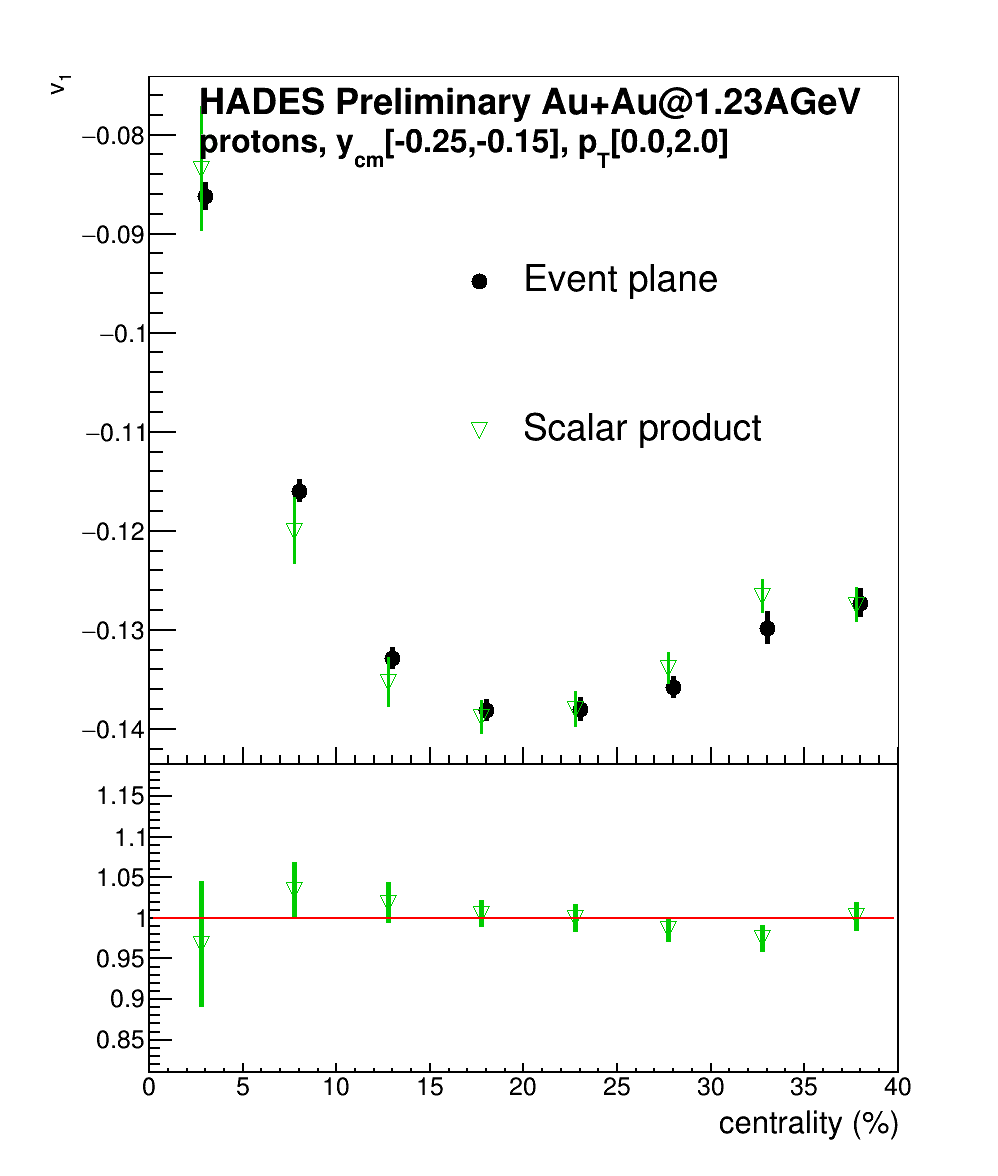
\includegraphics[width=0.45\linewidth]{images/EP_vs_SP.png}
\caption{Направленный поток протонов $v_1$, рожденных в столкновении Au+Au при энергии $E_{kin}=$1.23$A$~ГэВ как функция центральности столкновения. Результаты показаны для методов скалярного произведения (SP) и плоскости события (EP).}
\label{fig:hades_ep_vs_sp}
\end{center}
\end{figure}

\subsection{Сравнение методов случайных подсобытий и метода трёх подсобытий}

На рис.~\ref{fig:hades_rs_3s} показан направленный поток $v_1$ протонов, рожденных в столкновении Au+Au при энергии $E_{kin}=$1.23$A$~ГэВ (слева), Ag + Ag при энергии $E_{kin}=$1.23$A$~ГэВ (посередине) и Ag + Ag при энергии $E_{kin}=$1.58$A$~ГэВ (справа) как функция центральности столкновения. Результаты представлены для методов трех подсобытий и метода случайных подсобытий.
Для столкновений Au + Au при при энергии $E_{kin}=$1.23$A$~ГэВ (слева) разница между двумя методами вычисления корректировочного коэффициента разрешения составляет менее 5\% для среднецентральных столкновений.
Однако для меньшей системы столкновения, разница значительно больше. 
Это может быть объяснено меньшей множественностью рожденных частиц и спектаторов, и большим относительным вкладом непотоковых корреляций между $Q_1$-векторами, используемыми для расчета разрешения плоскости симметрии.
Наибольшая разница между двумя методами наблюдается для столкновений Ag + Ag при энергии $E_{kin}=$1.58$A$~ГэВ (справа).
Этот факт объясняется меньшим значением направленного потока $v_1$ спектаторов, отсюда больший относительный вклад непотоковых корреляций.
На основании этого наблюдения, можно сделать вывод о ненадёжности метода случайных подсобытий для более лёгких систем.
%
\begin{figure}[ht]
\begin{center}
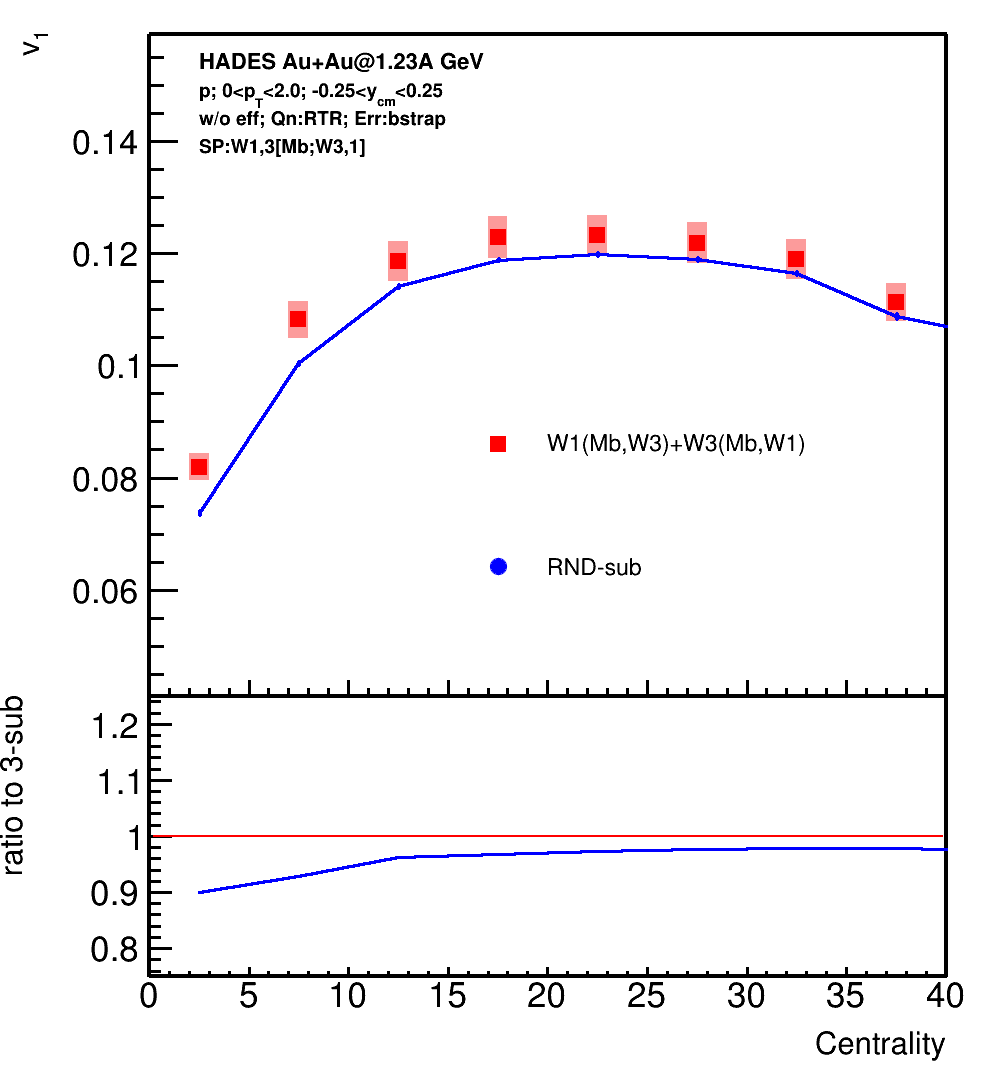
\includegraphics[width=0.3\linewidth]{images/v1_au123_3s_rnd.png}
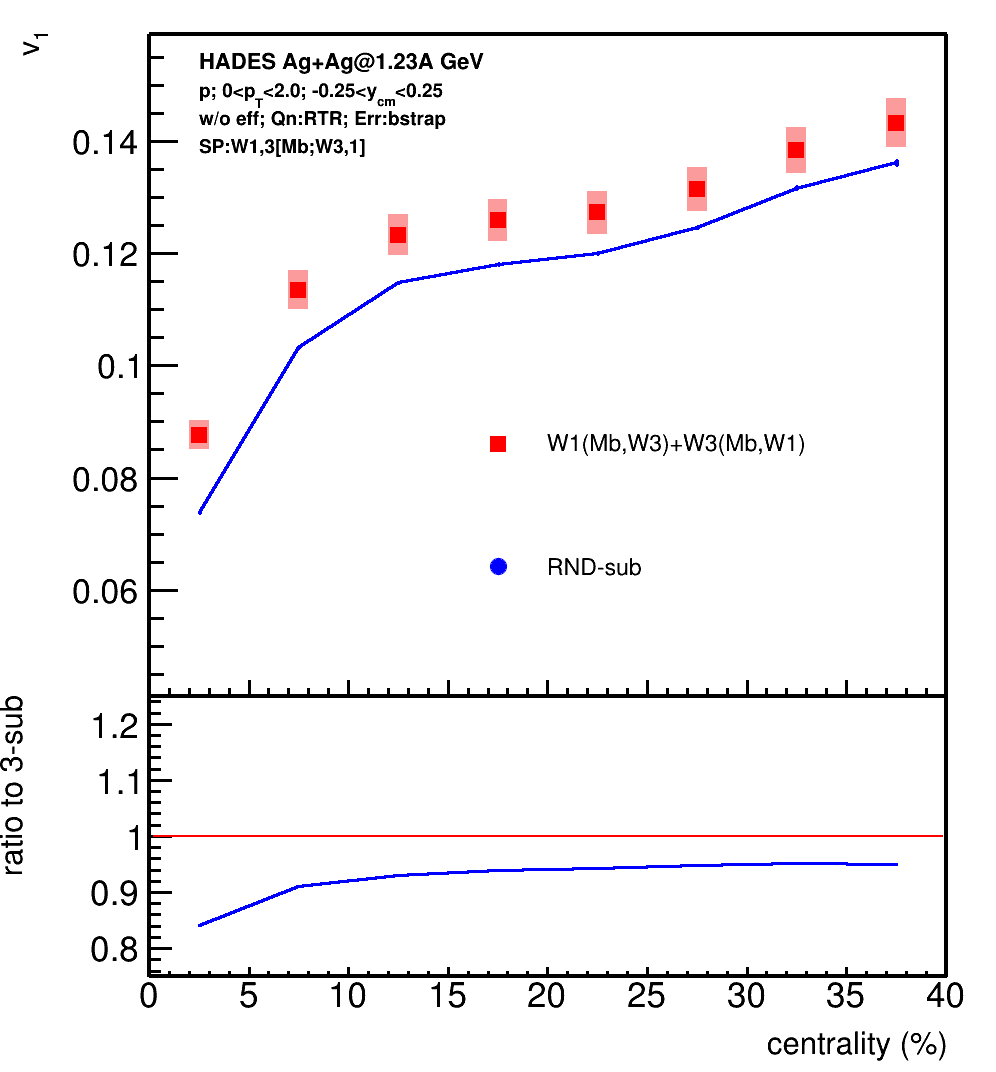
\includegraphics[width=0.3\linewidth]{images/v1_ag123_3s_rnd.png}
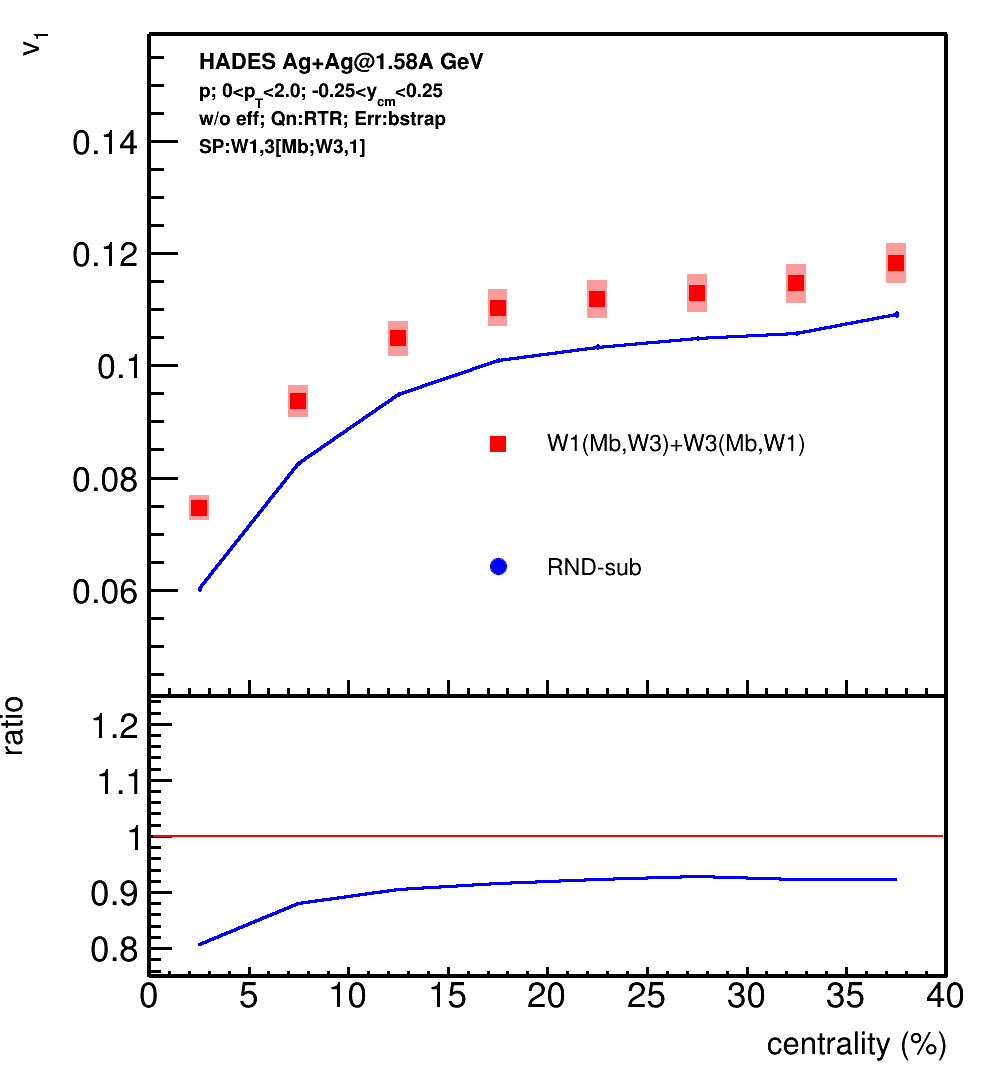
\includegraphics[width=0.3\linewidth]{images/v1_ag158_3s_rnd.png}
\caption{Направленный поток $v_1$ протонов, рожденных в столкновении Au+Au при энергии $E_{kin}=$1.23$A$~ГэВ (слева), Ag + Ag при энергии $E_{kin}=$1.23$A$~ГэВ (посередине) и Ag + Ag при энергии $E_{kin}=$1.58$A$~ГэВ (справа) как функция центральности столкновения. Результаты показаны для методов трех подсобытий и метода случайных подсобытий.}
\label{fig:hades_rs_3s}
\end{center}
\end{figure}

\subsection{Оценка итоговой систематики в значения $v_1$ от непотоковых корряляций}


На рис.~\ref{fig:hades_v1_publ_comparison} представлено сравнение направленного потока измеренного для столкновений Au + Au при энергии $E_{kin}$=1.23$A$~ГэВ с опубликованными данными~\cite{HADES:2020lob}.
Направленный поток $v_1$ как функция быстроты (слева) и поперечного импульса (справа) хорошо согласуется с опубликованной зависимостью для протонов.
Получение независимого измерения направленого потока $v_1$ и вычисленные значения ошибки из-за непотоковых корреляций позволило коллаборации позволило опубликовать имеющиеся результаты.
%
\begin{figure}[ht]
\begin{center}
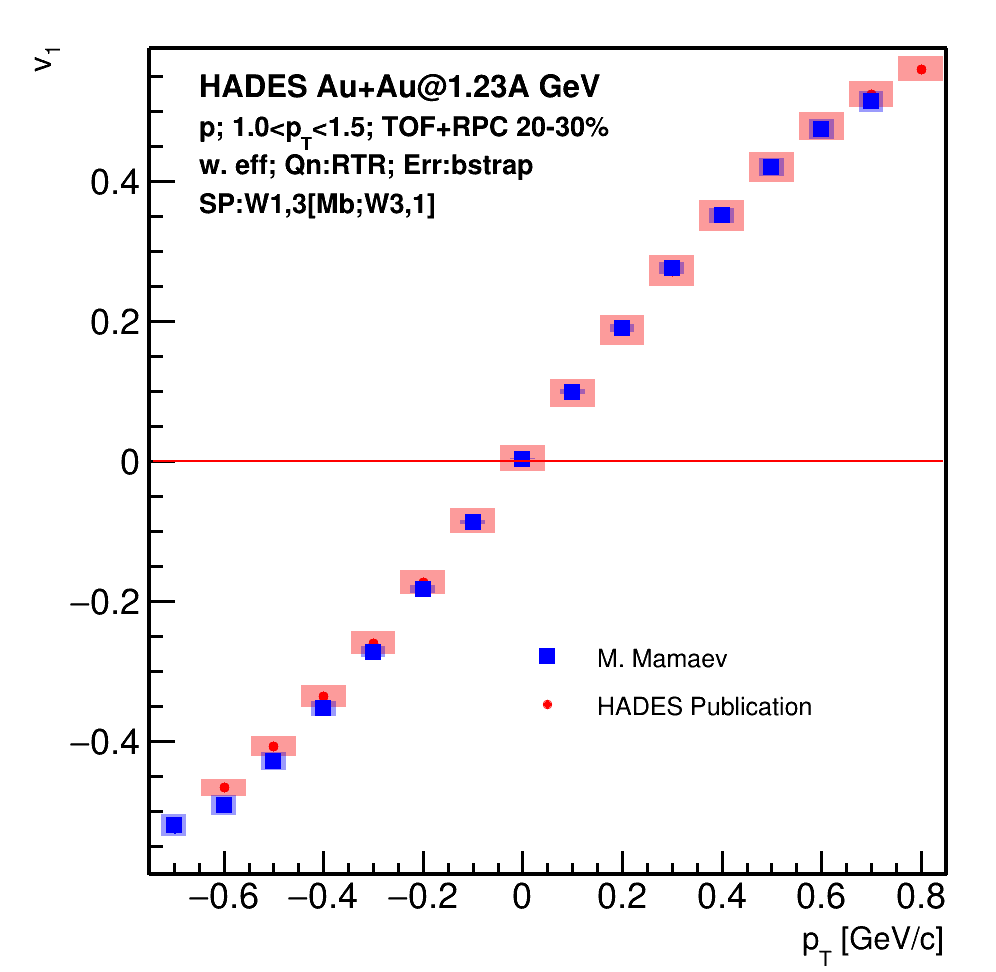
\includegraphics[width=0.45\linewidth]{images/v1_au123_publication_ycm.png}
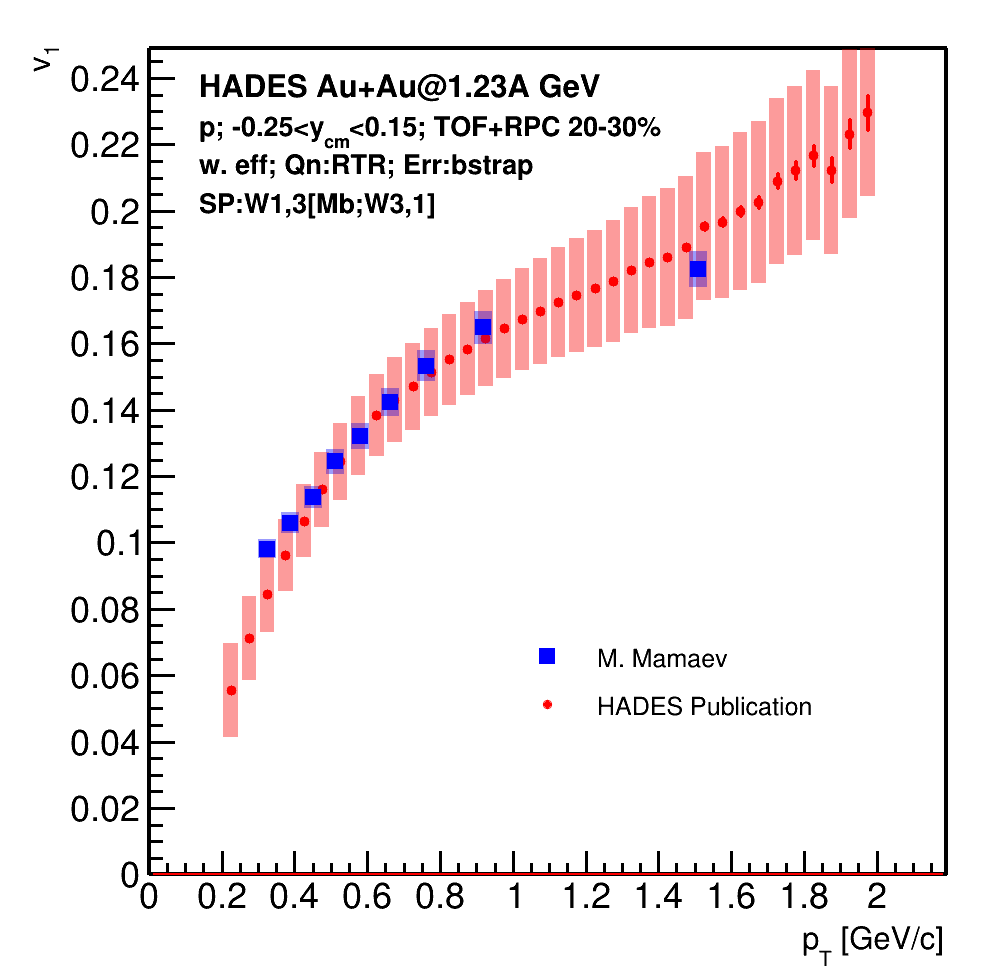
\includegraphics[width=0.45\linewidth]{images/v1_au123_publication_pT.png}
\caption{Направленный поток ($v_1$) протонов  рожденных в столкновении Au+Au при энергии $E_{kin}=$1.23$A$~ГэВ как функция быстроты (справа) и поперечного импульса (слева). Сравнение полученных результатов с опубликованными данными~\cite{HADES:2020lob}. }
\label{fig:hades_v1_publ_comparison}
\end{center}
\end{figure}

